\documentclass{article}

% if you need to pass options to natbib, use, e.g.:
%     \PassOptionsToPackage{numbers, compress}{natbib}
% before loading neurips_2020

% ready for submission
% \usepackage{neurips_2020}

% to compile a preprint version, e.g., for submission to arXiv, add add the
% [preprint] option:
%     \usepackage[preprint]{neurips_2020}

% to compile a camera-ready version, add the [final] option, e.g.:
%     \usepackage[final]{neurips_2020}

% to avoid loading the natbib package, add option nonatbib:
\usepackage[nonatbib]{neurips_2020}

\usepackage[utf8]{inputenc} % allow utf-8 input
\usepackage[T1]{fontenc}    % use 8-bit T1 fonts
\usepackage{hyperref}       % hyperlinks
\usepackage{url}            % simple URL typesetting
\usepackage{booktabs}       % professional-quality tables
\usepackage{amsfonts}       % blackboard math symbols
\usepackage{nicefrac}       % compact symbols for 1/2, etc.
\usepackage{microtype}      % microtypography
% Added from ECCV
\usepackage{graphicx}
\usepackage{multirow}
\usepackage{subfigure}
% \usepackage{subtable}
\usepackage{amsmath}
\usepackage{floatrow}
\usepackage{caption}
\captionsetup[table]{position=bottom}   %% or below
\captionsetup[tabular]{position=bottom}   %% or below

\usepackage{bm}% bold math
\usepackage{amsmath}
\usepackage{subcaption}
\usepackage{url}
\usepackage{color}
\usepackage{mathrsfs}
\usepackage{amsthm}
\newtheorem{theorem}{Theorem}
\newtheorem*{theorem*}{Theorem}


\DeclareMathOperator{\softmax}{Softmax} 
%\title{Improving Semantic Segmentation through Label Propagation with Cyclic Label Consistency and Uncertainty}
%\title{Warp-Refine Propagation and Uncertainty-Aware Training for Semantic Segmentation}
\title{Improving Semantic Segmentation via Cycle-consistent Video Auto-labeling}
% On cycle consistency and noisy-label learning for semantic segmentation.
% Utilizing cycle consistency and aleatoric uncertainty for enhancing semantic segmentation.
% 
% Enhancing label propagation with cycle consistency, and improving noisy label learning by modelling uncertaint

% The \author macro works with any number of authors. There are two commands
% used to separate the names and addresses of multiple authors: \And and \AND.
%
% Using \And between authors leaves it to LaTeX to determine where to break the
% lines. Using \AND forces a line break at that point. So, if LaTeX puts 3 of 4
% authors names on the first line, and the last on the second line, try using
% \AND instead of \And before the third author name.

\author{%
  David S.~Hippocampus\thanks{Use footnote for providing further information
    about author (webpage, alternative address)---\emph{not} for acknowledging
    funding agencies.} \\
  Department of Computer Science\\
  Cranberry-Lemon University\\
  Pittsburgh, PA 15213 \\
  \texttt{hippo@cs.cranberry-lemon.edu} \\
  % examples of more authors
  % \And
  % Coauthor \\
  % Affiliation \\
  % Address \\
  % \texttt{email} \\
  % \AND
  % Coauthor \\
  % Affiliation \\
  % Address \\
  % \texttt{email} \\
  % \And
  % Coauthor \\
  % Affiliation \\
  % Address \\
  % \texttt{email} \\
  % \And
  % Coauthor \\
  % Affiliation \\
  % Address \\
  % \texttt{email} \\
}

\begin{document}

\maketitle

\begin{abstract}
% Aditya
Not only are Deep Learning models for semantic segmentation notably data-hungry, the dense manual annotation required for the task is also prohibitively costly. Automatically annotating video frames by propagating labels through time is a promising economical approach towards enriching training data and alleviating this data-bottleneck. We propose a novel label propagation method which leverages cycle consistency across time to propagate labels over significantly longer time horizons and with higher accuracy than previously possible. We also observe that dense pixel annotation, be it manual or automated, is a noisy process. To robustly train with labels from multiple noisy labeling processes, we derive a principled approach which aims to capture the label uncertainty. With our approach, we are able to effectively utilize labels from multiple noisy label distributions. We validate our contributions on the Cityscapes and ApolloScape datasets where we achieve \textit{state-of-the-art} results.

% Dennis's pass
% Deep Learning models for semantic segmentation are notably data-hungry, as manual annotation is labor-intensive. Automatically annotating video frames by propagating labels through time is a promising approach for enriching training data. Leveraging cycle consistency across frames, we propose a novel label propagation method which can propagate labels over significantly longer time horizons and with higher accuracy than previously possible. We also observe that dense pixel annotation, be it manual or propagated, is a noisy process. To robustly train with noisy labels, we derive a principled approach whereby we aim to capture the uncertainty inherent in various label generation processes. The model learns how to effectively combine labels from multiple noisy label distributions with explicit uncertainty modelling. We validate our contributions on the Cityscapes and ApolloScape datasets where we achieve \textit{state-of-the-art} results.

% 
%%% Rares's pass
%Deep Learning models for semantic segmentation are notably data-hungry, with labels expensive and difficult to acquire. Automatically labeling data through label propagation is a promising approach for improving the performance of such models. Leveraging cycle consistency, we propose a novel label propagation method which is able to propagate labels over longer time horizons and with significantly less noise than previously possible. Our second insight comes from the fact that labeling, be it manual or propagated, is a noisy process. To account for this, we derive a principled approach whereby we aim to capture the uncertainty inherent in various label generation processes. By explicitly modeling this uncertainty, we learn how to effectively combine labels from multiple noisy label distributions. We validate our contributions on the Cityscapes and ApolloScape datasets where we achieve \textit{state-of-the-art} results.



%%% OLDER ABSTRACT
%In the spectrum of semi-supervised methods, label propagation stands out as a very promising candidate for improving semantic segmentation, especially in the domain of autonomous driving, where data is traditionally collected in a temporal sequence. 
% Deep Learning models for semantic segmentation are notably data-hungry. Automatically labeling additional data through label propagation is a promising approach for improving the performance of such models.
% In this paper, we address two fundamental aspects of this approach: the quality of propagated labels, and the drawbacks of learning with noisy propagated labels. 
% First, we propose a new method called Warp-Refine Propagation which, by leveraging the consistency of labels in a cyclic propagation loop, significantly improves the propagated labels.
% Our method refines labels generated from optical flow-based methods by learning to inpaint and denoise them. With our method, we are able to propagate labels for much longer, and with significantly less noise, generating diverse, and useful training data. 
% However, the generated labels are inherently noisy, curtailing the performance of deep models trained with them. Hence, we propose a principled approach, namely Uncertainty-Aware-Training for training with noisy labels. The noise in generated labels is handled by modelling label uncertainty from the labelled data itself.
% As our approach is independent of the label generation process, we can tackle multiple noisy label distributions at the same time.
% The labels generated from our method, together with the modelling of label uncertainty, allow us to achieve %\textit{state-of-the-art}
% competitive
% performance for the Cityscapes and ApolloScape datasets. 

% , especially in the domain of autonomous driving, where data is traditionally collected in a temporal sequence. 
% Previous \textit{state-of-the-art} approach for label propagation utilizes optical-flow based warping between image frames to propagate labels, yielding noisy propagated labels. In this work, we propose a novel method \textit{LP-MID: Label Propagation with Masking, Inpainting and Denoising} to significantly improve propagated labels. Our method refines labels generated from optical-flow based warping by learning to inpaint and denoise such labels in a supervised manner. At the heart of our approach lies the consistency of labels in a cyclic propagation loop. With our method, we are able to propagate labels for much longer, and with significantly less noise, generating more diverse, and useful data for training. 
% This is particularly useful in the case of data-scarcity. 
% Further, by leveraging the epistemic uncertainty of the propagated labels, we propose a selective learning policy, which specifically addresses the drawbacks of models trained without propagation. Using our method we achieve \textit{state-of-the-art} performance on Cityscapes dataset of $100$ mIOU. %, and on Apolloscapes dataset of $100$ mIOU. 
% Finally, we also show the significant benefits of our approach in the case of data scarcity. Our method  achieves a m$\%$ improvement over supervised training baselines, when only $15$ \% of labelled data is used.

\end{abstract}


\section{Introduction}
\label{section-intro}


While deep learning has enabled highly performative modeling for various computer vision tasks~\cite{sota_imclass, sota_objdet}, large quantities of annotated data are still required for achieving \textit{state-of-the-art} performance~\cite{alex2019big}. This predicament is further exacerbated for tasks such as semantic segmentation, where the dense pixel-level annotations required for training can be prohibitively expensive. Various semi-supervised~\cite{semi_aug_2, domain_seg_nips_2, semi_sup_seg_1}, and self-supervised methods~\cite{self_sup_aaai, self_sup_iccv} have been proposed to alleviate this data-bottleneck, however they bring their own set of challenges such as domain-shift.

While dense annotation is costly~\cite{benenson2019large,kuznetsova2018open,cs_dataset}, collecting raw sequential image data is relatively cheap. This is especially the conventional methodology for autonomous driving datasets, such as~\cite{cs_dataset, as_dataset, argo_dataset}. Such datasets are often sparsely annotated across time (for example, in~\cite{cs_dataset}, pixel-level segmentation is provided once in every continuous partition of 30 frames). To assuage the data bottleneck, we can generate approximated labels for the unlabelled samples. 
While weak labels can be generated via \textit{lazy labelling}~\cite{lazy_label}, or pseudo-semantic annotations~\cite{taskonomy2018,pseudo_nips_1}, 
 the presence of an annotated sample in a continuous temporal sequence motivates the use of label propagation~\cite{lp_2006, lp_2010} for generating the approximated labels of neighbouring frames. 
 
\let\clearpage\relax
	\begin{figure}[t]
		\label{fig:comparison}
		\centering
		\subfigure[We propose a novel approach for propagation as well as training.]
		{
			\begin{minipage}{0.65\textwidth}
				\centering
				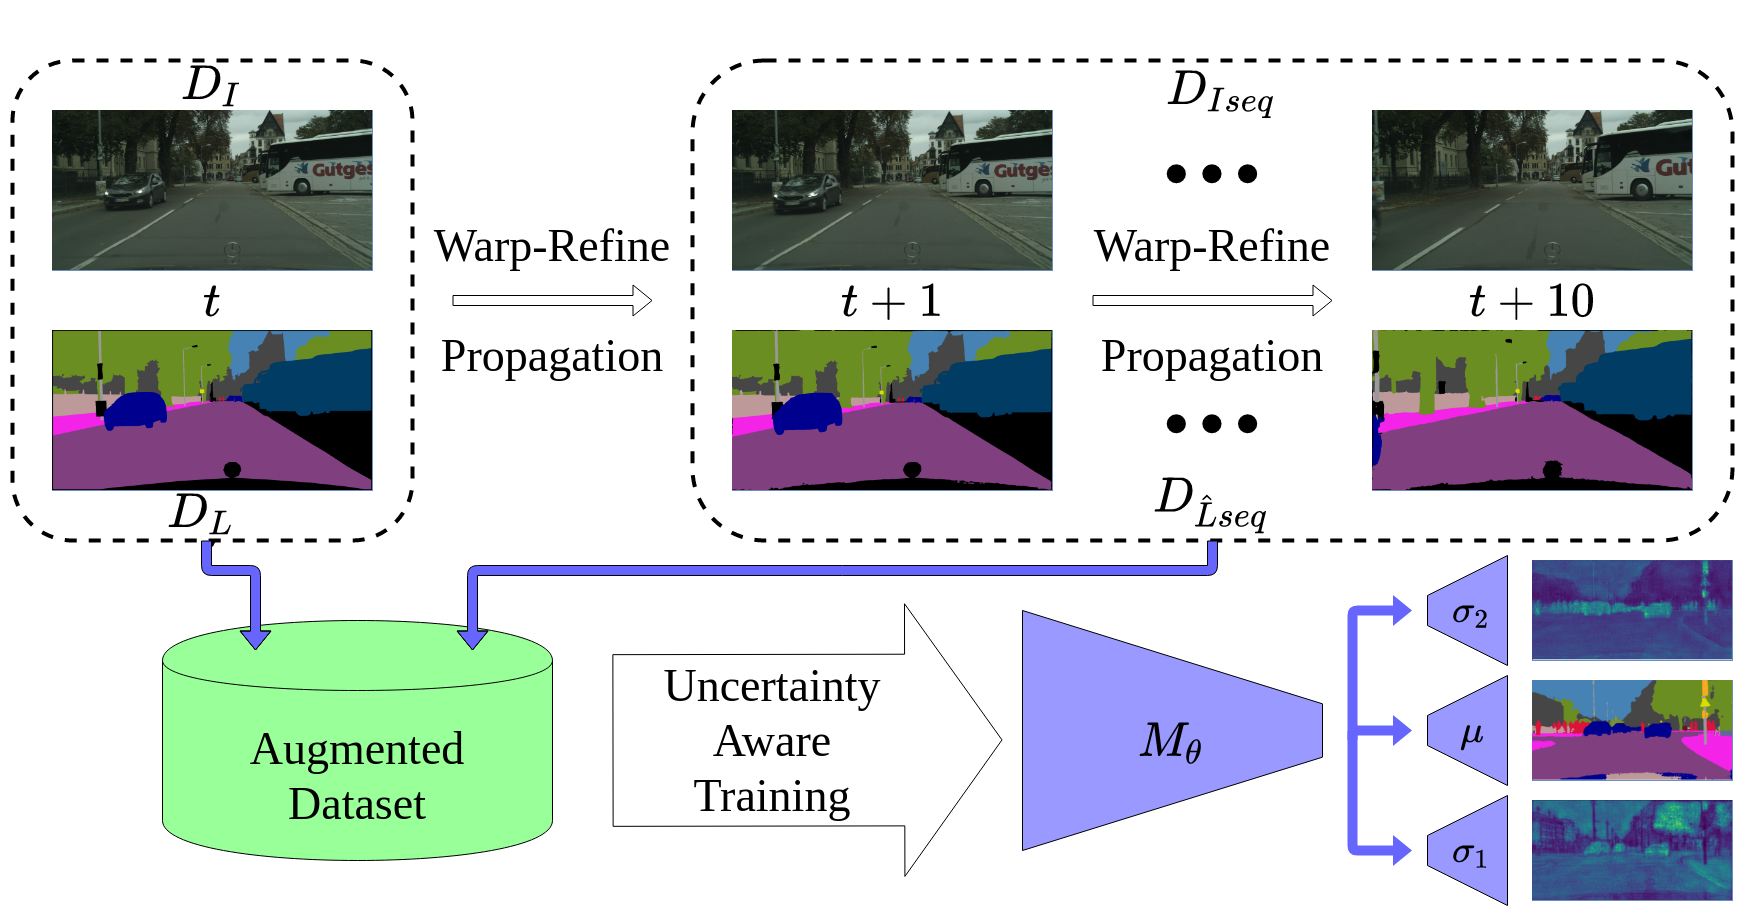
\includegraphics[width=1.0\linewidth]{figures/overview_lr.png}
				\vfill
			\end{minipage}
		}
		\hfill
        \hspace{-2em}
		\subfigure[Top:~\cite{nvidia_cvpr19}, Bottom: Ours]
		{
            % \begin{minipage}[b][0.315\textheight][s]{0.315\textwidth}
            \begin{minipage}{0.33\textwidth}
% \subfloat[(a)]{%
%   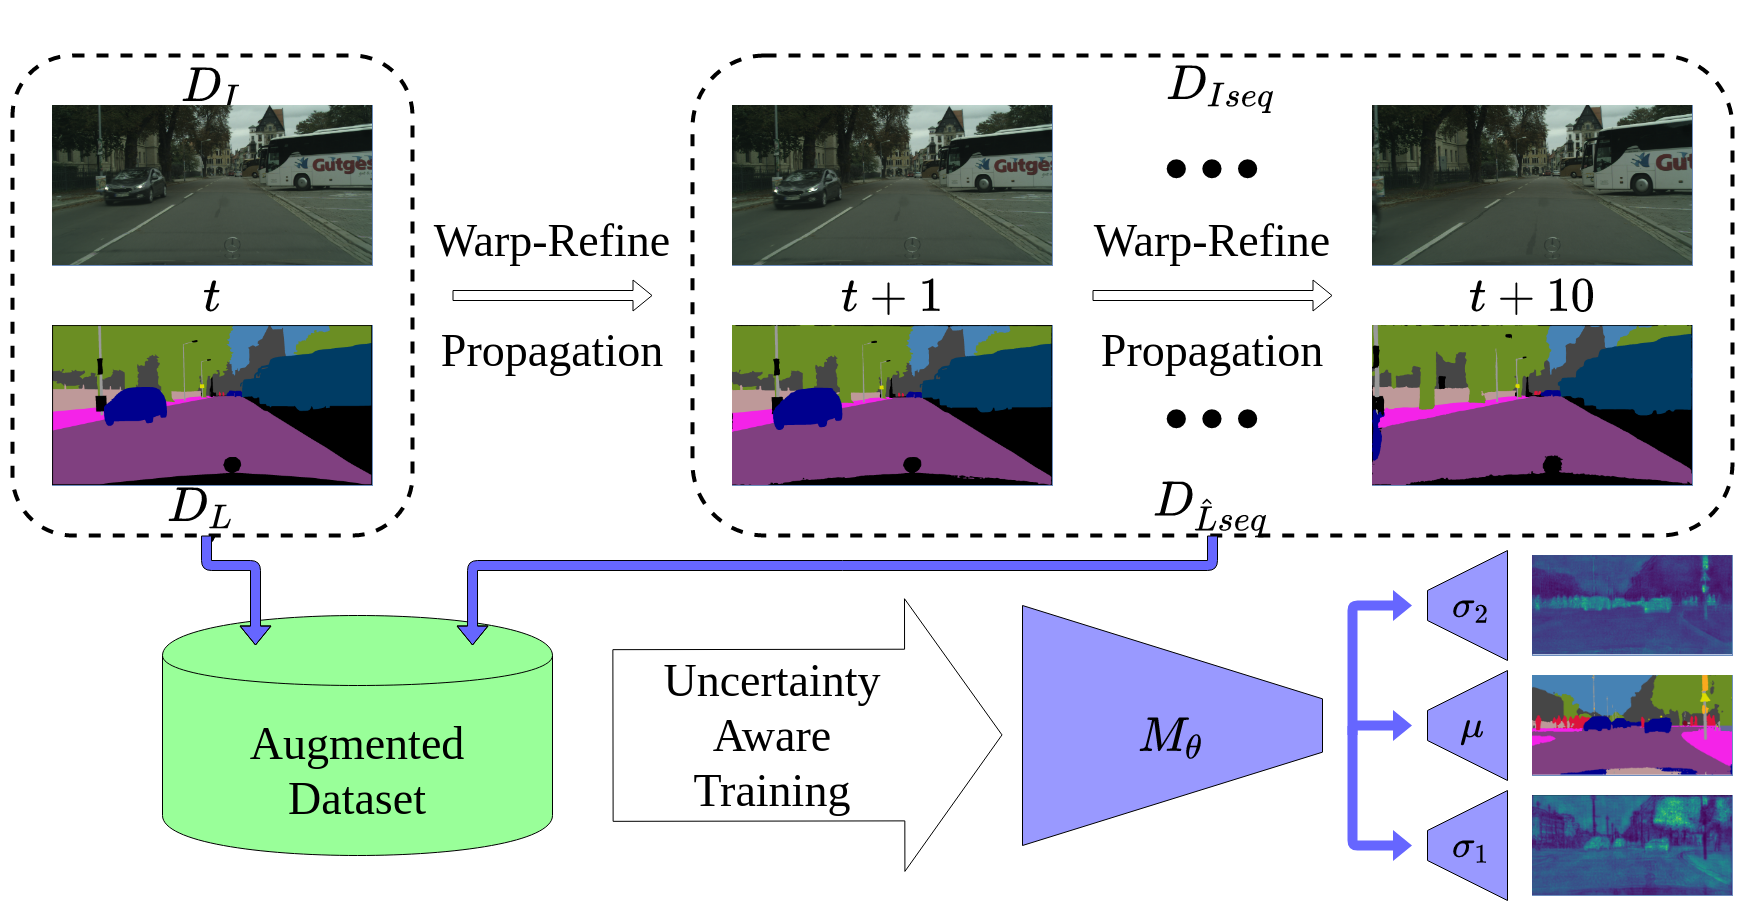
\includegraphics[clip,width=0.315\textwidth]{figures/fig_overview_lowres.png}%
% }
% \subfloat[(b)]{%
%   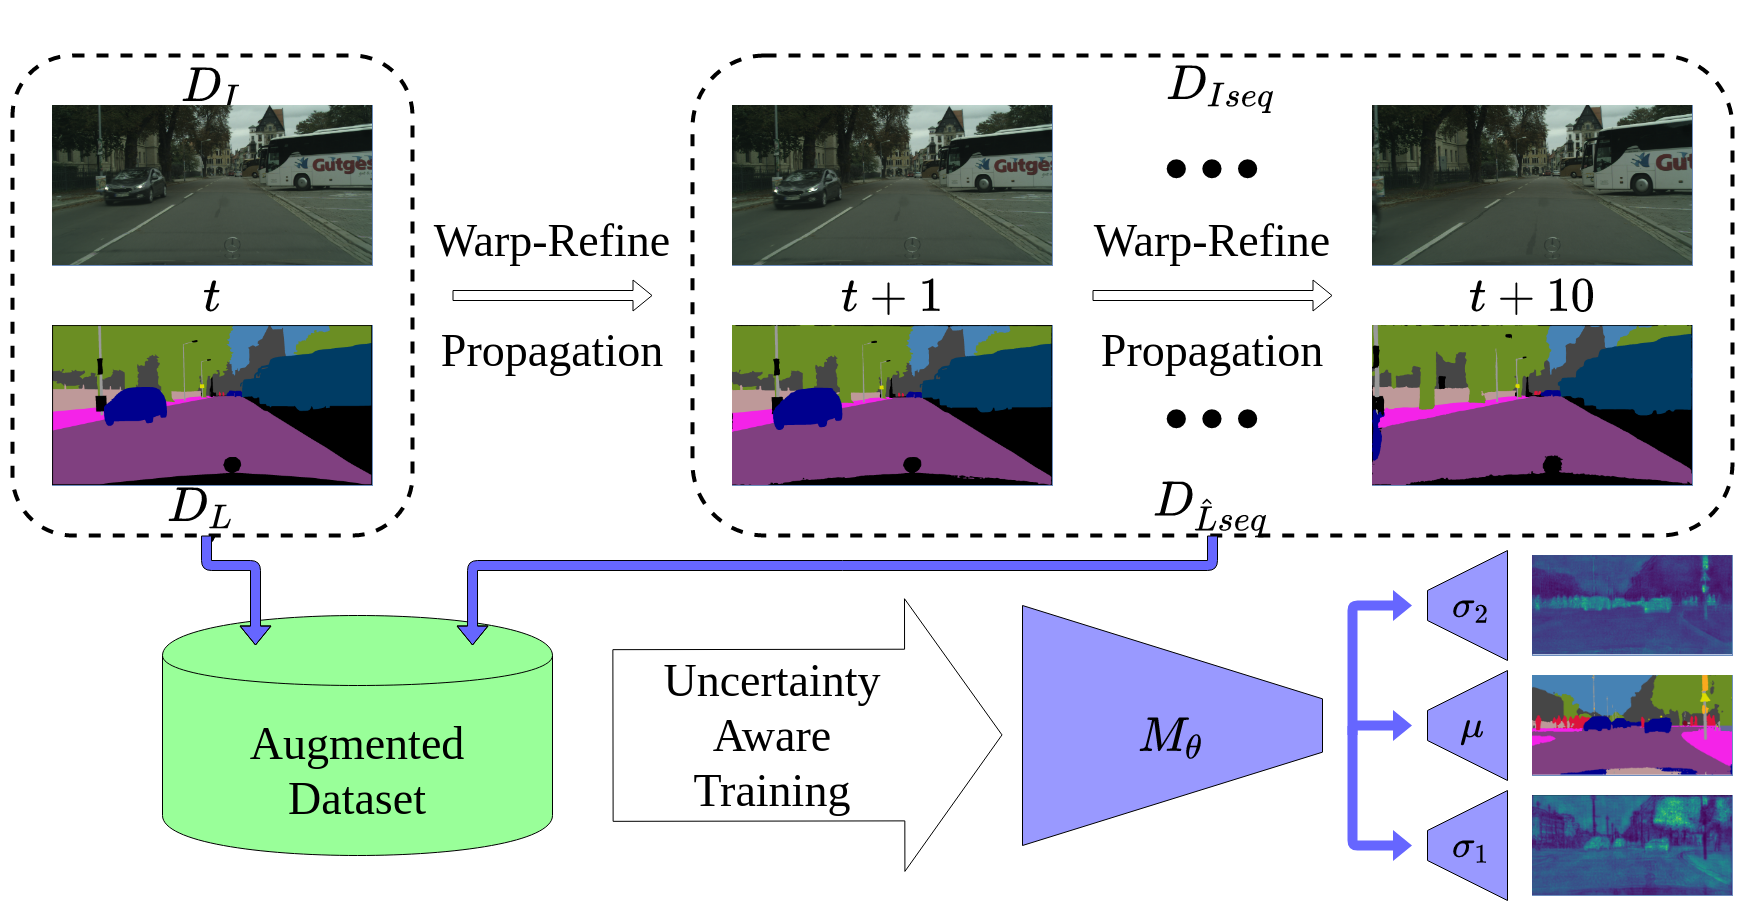
\includegraphics[clip,width=0.315\textwidth]{figures/fig_overview_lowres.png}%
% }
				\centering
				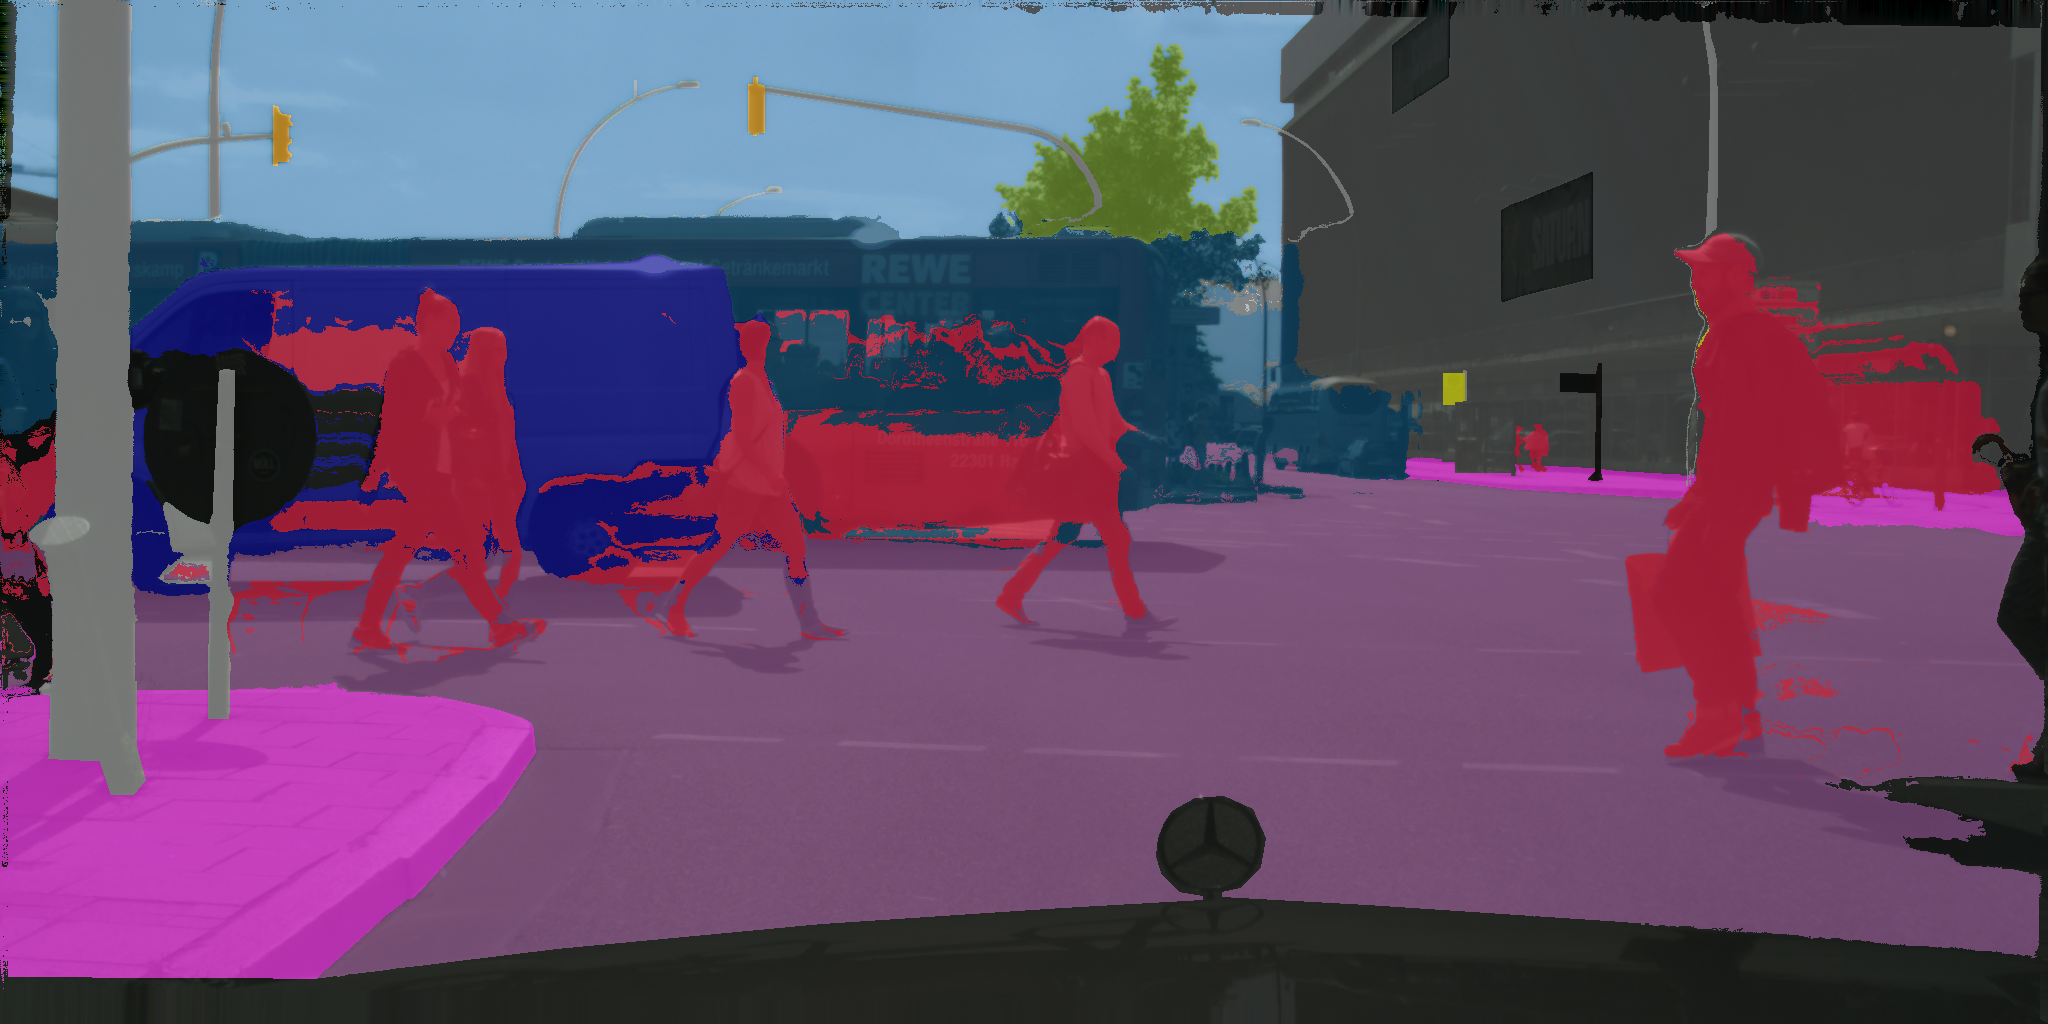
\includegraphics[width=\textwidth]{figures/prev_2.png}
				\vfill
				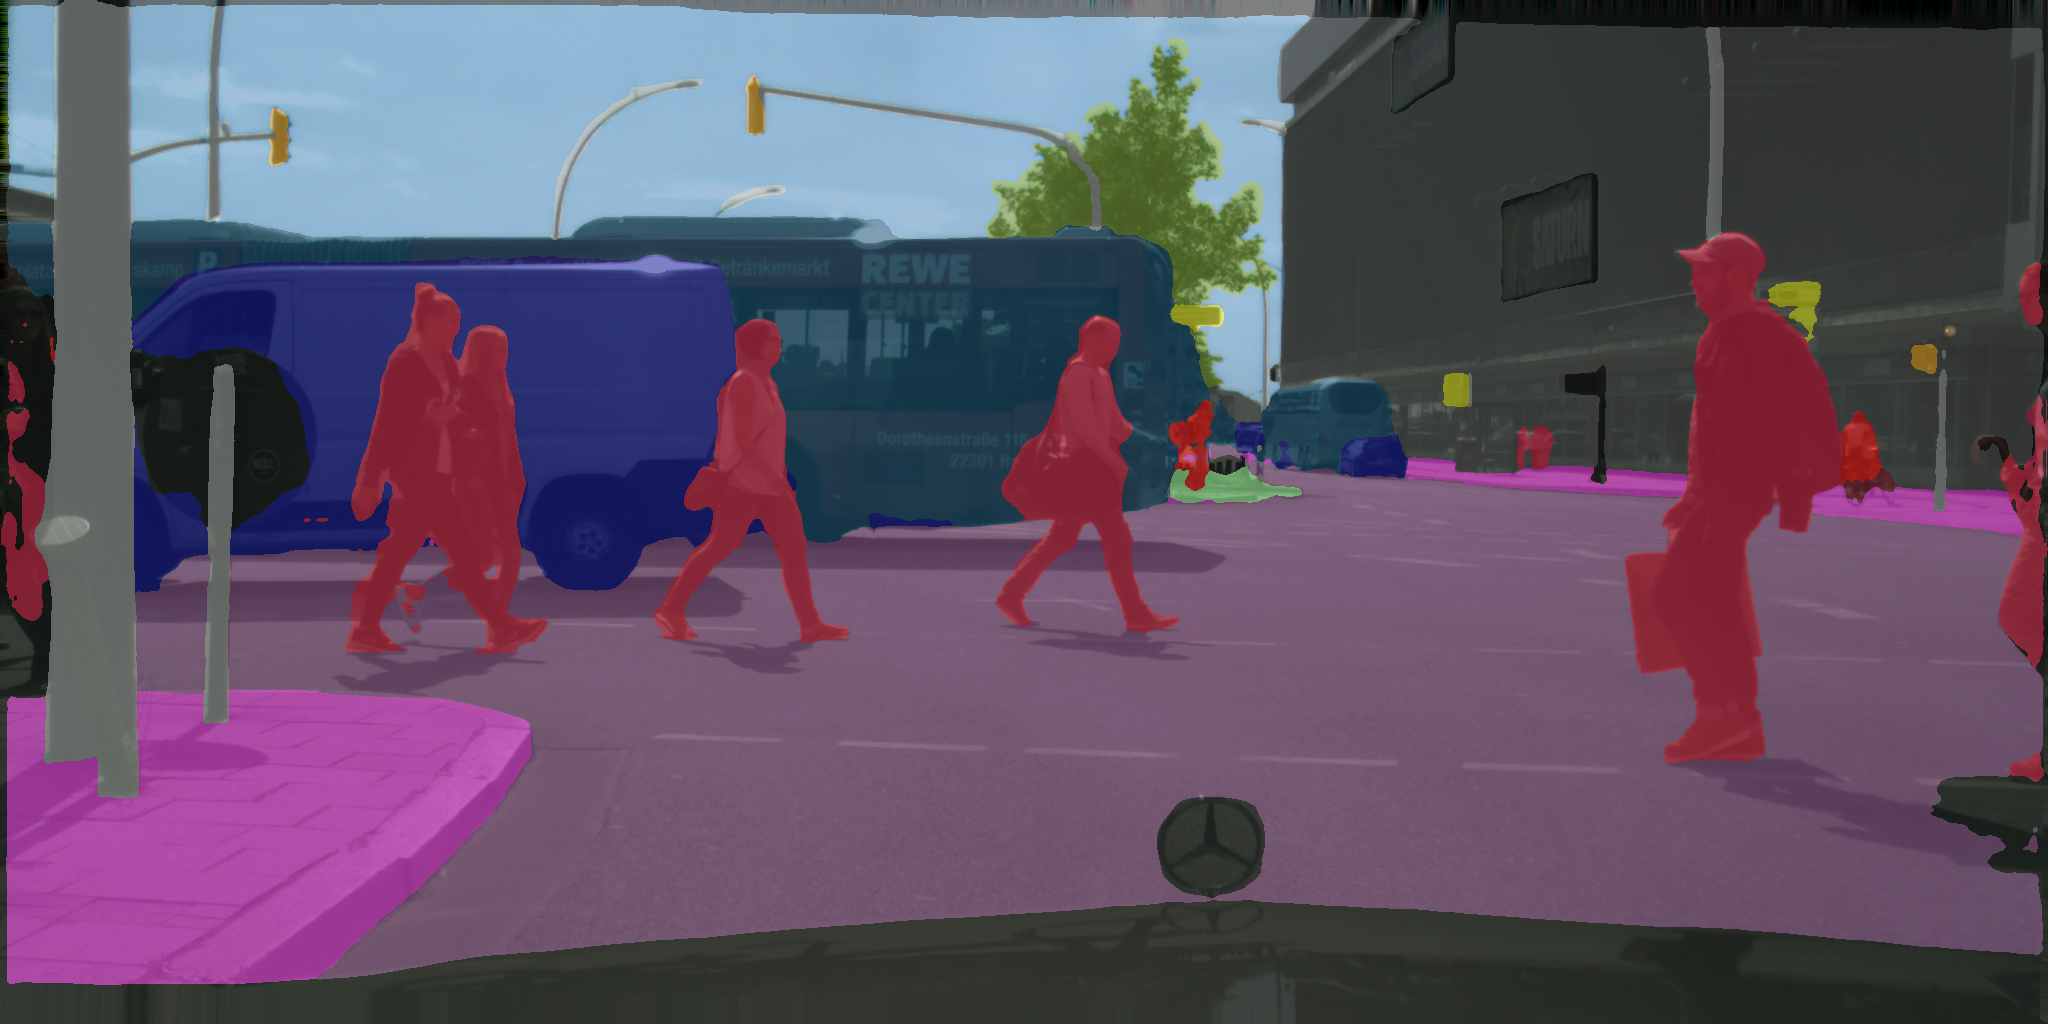
\includegraphics[width=\textwidth]{figures/our_2.png}%
				\vspace{0.3em}
			\end{minipage}
		}
    \vspace{-0.5em}
		\caption{\small (a) Using our propagation method, we generate pseudo-labels for images $D_{Iseq}$. The generated and the clean labels are then used for uncertainty-aware-training of semantic segmentation models. (b) Our method significantly surpasses \textit{state-of-the-art} label propagation methods~\cite{nvidia_cvpr19}.
		}
		\vspace{-0.5em}
	\end{figure}


The two primary concerns regarding label propagation are: a) \textit{How to perform it?} and b) \textit{How to utilize the generated labels?} In this work, we address both: We propose a new method to improve label propagation, and a principled approach for training with generated noisy labels. 

% The current \textit{state-of-the-art} method [], utilizes a \textit{video-reconstruction} model for label propagation. 
% The model, given the labelled image and its adjacent image, estimates a warping function from the labelled image to the adjacent image. The same estimated warping function, which is in the form of pixel-level motion vectors, is then applied to the labels to yield \textit{pseudo-labels} for the adjacent image. 
% By employing this model recurrently on a image sequence, the authors propagate labels to images further apart from the labelled image. However, 
Previous methods~\cite{lp_iccvw, lp_eccv, nvidia_cvpr19}, due to their reliance on geometric cues, have several of the same drawbacks as that of optical flow estimation. Specifically, prominent features of real-world data such as the lack of brightness consistency, or large motions, introduce harmful noise in the propagated labels. This drawback is further aggravated by the accumulation of errors as labels are propagated further in time. This is crucial, as longer propagation can yield more diverse labelled data, which is more beneficial for training deep neural networks~\cite{lp_eccv}.

Specifically, we make two important observations w.r.t previous propagation methods~\cite{lp_eccv, nvidia_cvpr19}: 1) They do not leverage the semantic knowledge in the annotated dataset, and 2) The noise in labels propagated with geometric methods has a systemic component which can be modelled. We propose a new propagation method called \emph{Warp-Refine Propagation} addressing both of these concerns. This method consists of two steps, a label warping step followed by a label refinement step. At the heart of our approach is the concept of cyclic consistency of labels, which we explain in detail in Section~\ref{subsec-alea}. As shown in Figure~\ref{fig:comparison}, our method significantly outperforms previous methods. 

In spite of the improvements, the propagated labels can still be noisy, especially when propagation takes place for larger time steps. 
% This is problematic as deep network can memorize noise in labels, leading to poor generalization~\cite{noisy_memory}.
% Furthermore, the noise does not allow us to use propagated labels which are further away, and contain more novel information. 
To address this challenge, we formulate \emph{Uncertainty-Aware Training}, a principled approach for training with noisy labels which contrasts previous heuristic methods such as label relaxation~\cite{nvidia_cvpr19} or loss weighting~\cite{lp_eccv}. 
We train the model to estimate the probability of the noisy labels under the true label distribution. This allows us to estimate the uncertainty of each label generation process, mitigating the drawbacks of training with noisy labels.
% Further, we provide theoretical proof that our approach implicitly reduces the total variational distance between the model and the true underlying distribution.
% In brief, we model the relation between noisy labels and the true labels in the form of label uncertainty, which alleviates the drawbacks of training with noisy labels. 
Furthermore, our approach can be used for multiple noisy distributions at the same time. Hence, with minimal changes to our model, we are also able to use pseudo-labelling~\cite{taskonomy2018,pseudo_nips_1}, i.e. noisy predictions from a pretrained-model, for data points where propagation is not possible. 
%In section~\ref{subsec-alea}, we draw the link between our approach and modelling of aleatoric uncertainty~\cite{gal_main} for different data generation processes. 

By using our propagation method, and our noisy label learning approach, we are able to achieve \textit{state-of-the-art} performance for two large scale autonomous driving datasets, namely Cityscapes, and ApolloScape. Further, we provide quantitative evaluation of various propagation methods which has crucially been missing from previous literature.

In summary, we 
\begin{itemize}
    \item Improve label propagation with a new approach called \emph{Warp-Refine Propagation}, and provide quantitative as well as qualitative evaluation for the same. 
    \item Propose \emph{Uncertainty-Aware Training}, a principled approach for learning with noisy labels, for which we further provide theoretical justification.
    \item Utilize our proposed advancements to achieve \textit{state-of-the-art} performance for two real-world autonomous driving datasets.
\end{itemize}



% TO BE SHORTENED.

\section{Related Works}
\label{section-rel}


\cite{fcn_cvpr, rcnn_1} were one of the first works to introduce deep architectures for the task of semantic segmentation. %, surpassing previous non-deep methods~\cite{non_deep_sem_seg, non_deep_sem_seg_2}. 
Multiple generations of work~\cite{deeplab_v1, deeplab_v2, pspnet, unet}, have further improved the performance, albeit at the cost of more computation mode labelled data requirement. A large corpus of previous literature alleviates the data bottleneck via semi-supervised approaches~\cite{semi_sup_seg_1, semi_sup_seg_2}, domain adaptation~\cite{domain_seg_1, domain_seg_2, domain_seg_3, domain_seg_nips_1, domain_seg_nips_2, multi_domain_seg}, and data augmentation~\cite{semi_aug_1, semi_aug_2}.

Works such as~\cite{noisy_self}, assuage the label bottleneck via creation of pseudo-labels for a large set of unlabelled images. This pseudo-labelling utilizes the semantic knowledge in the labelled dataset. In contrast, works such as~\cite{lp_eccv, lp_iccvw, lp_2013} propose label propagation, where geometric approaches such as video-prediction~\cite{sdc_net}, are utilized for generating labels.
%In such works, the geometric knowledge is utilized for generating pseudo-labels. 
To the best of our knowledge, our work is the first to utilize both the semantic and geometric understanding to propagated labels.
%Mention gal\_multitask.
The combination of semantic and geometric understanding has been explore in the past for other tasks~\cite{future_seg, sem_warp, feelvos2019}. Our chief distinction is the propagation of ground-truth labels, which in turn necessitates a novel cyclic label consistency-based loss. 
%Furthermore, since our process can be performed offline, lack of compute bottleneck allow us to explore highly performative modeling inspired from recent generative modelling methods~\cite{pix2pix, spades}. 
The concept of cyclic consistency has been used previously for learning object embeddings~\cite{CVPR2019_CycleTime}, and video interpolation~\cite{cycle_vid_interp}. Our work is inspired from~\cite{CVPR2019_CycleTime}, where cyclic consistency is used for learning object embeddings using a robust tracker. However, unlike~\cite{CVPR2019_CycleTime}, we address the noisy nature of our tracking/geometric modelling method itself.

Previous works deal with the noise in propagated labels by defining heuristics such as trust-factor~\cite{lp_eccv} or label-relaxation~\cite{nvidia_cvpr19}. In our work, we propose a principled approach based on modelling the label uncertainty. Recently,~\cite{gal_main, gal_multitask, uncer_nips_2, uncer_nips_3} have explored modelling of uncertainty in the context of deep learning models. Furthermore, works such as~\cite{uncer_label_1, uncer_label_2}, have explored the relation between aleatoric uncertainty, and label noise. In~\cite{uncer_label_1}, the authors propose a sophisticated noise model for dealing with noisy labelling in the task of keypoint matching. While we also utilize aleatoric uncertainty for dealing with label noise, our approach is formulated for handling multiple noisy label distributions at the same time with minimal computational overhead, unlike~\cite{uncer_label_1}.


\section{Methodology}
\label{section-method}

In this section we describe our approach in detail. Section~\ref{subsec-lw} defines our warping module, Section~\ref{subsec-lr} describes the label refinement module, and Section~\ref{subsec-alea} describes our noisy label learning approach.


\textbf{Problem Formulation}: We have a set of images $D_{I}$ and the corresponding labels $D_{L}$. We also have a set of images $D_{Iseq}$ consisting of images temporally adjacent to images in $D_{I}$. 
% Specifically, for each $I_{t}^{i} \in D_{I}$, the set of images $\{I_{t-x}^{i} | -p\leq x \leq p\}$ is a partition of $D_{Iseq}$. Here, $I \in \Bbb R ^{n \times w \times h}$, and the sub-script $t$ corresponds to temporal position in a video stream. 
Our goal is to generate the corresponding set of pseudo-labels, $\hat{D}_{Lseq}$. Using the generated pseudo-labels, our network can be trained on $D_{I}$ and $D_{Iseq}$, using corresponding labels from $D_{L}$ and $\hat{D}_{Lseq}$.

\subsection{Label Warping}
\label{subsec-lw}
The goal of this step is to generate warped labels $ \{\hat{L}^{w}_{n} | t\leq n \leq t + p\}$, where $p \in \mathbb{N}$ is a fixed integer, given the sequence of images $\{I_{n}| t\leq n \leq t + p\}$, and the annotated label $L_{t}$. In this step, we utilize a previous existing method~\cite{nvidia_cvpr19} for generating the warped labels. % We present a generalized formulation of this step.

% We now describe this system. 
% For the sake of simplicity, we drop the superscript $i$ denoting an image instance. 
We train a neural network $f_{\theta}$ such that, given a sequence of images $I_{t:t+x} = \{I_{n}| t\leq n \leq t + x\}$ it predicts parameters for the sampling and warping function $ \Phi$ to construct $I_{t+x}$ from $I_{t + x -1}$.
The pseudo-labels corresponding to $I_{t+x}$ can similarly be constructed by using the same function $\Phi$ on $\hat{L}^{w}_{t+x-1}$. For the sake of simplicity, we rewrite $I_{t:t+x}$ as the pair of images $(I_{t+x-1},I_{t+x})$. This step can be simply summarized as:

\begin{equation}
\label{eq-warp_gen}
    \Phi_{(t+x-1, t+x)} = f_\theta (I_{t+x-1}, I_{t+x}),
\end{equation}
\begin{equation}
\label{eq-warp_both}
    \hat{I}^{w}_{t+x} = \Phi_{(t+x-1, t+x)} ( \hat{I}^{w}_{t+x-1}) \quad;\quad \hat{L}^{w}_{t+x} = \Phi_{(t+x-1, t+x)} ( \hat{L}^{w}_{t+x-1}),
\end{equation}

where, we use $\hat{L}^{w}_t = L_t$ and $\hat{I}^{w}_t = I_t$. By using this method sequentially for $1 \leq x \leq p$, we can generate the warped labels $\hat{L}^{w}_{n}$ for all $t \leq n \leq t + p$.
This method exploits geometric information by predicting motion vectors for each pixel. A more detailed explanation can be found in~\cite{nvidia_cvpr19, sdc_net}. This method is prone to generating noisy labels due to errors in the estimation of the warping function $\Phi$. 

\textbf{Mask Inpainting}: We first introduce a simple post-processing step (named $\mathtt{MI}$) to enhance the warped labels, the goal being to identify regions where warping has failed, and to replace labels for such regions with other approximation strategies. 
% The presence of the reconstructed image $\hat{I^{w}}$, and the real image $I$ offers us a rather simple yet effective method to identify such regions. 
We measure the per-pixel distance between $\hat{I}$ and $I$ at each pixel $(x,y)$, and if it is higher than a fixed threshold $\tau$, we replace those labels with labels from a semantic segmentation network $S$ trained using $D_I$ and $D_L$. 
% This allows us to address propagation errors, and at the same time utilize semantic knowledge present in the annotated dataset. 
This is summarized as:

\begin{align}
\begin{split}
\label{eq-inpaint}
M(x, y) & = \mathbb{I}_{M}\big(d(\hat{I}(x,y),I(x,y) ) \leq \tau \big) \\
\hat{L}^{MI} & = \hat{L}^{w} \odot M + (1-M) \odot \hat{L}^{pred}
\end{split}
\end{align}
%The authors further propose \textit{joint-propagation}, replacing each $I_{t+1:t+p}$ in $D_{Iseq}$ with the warping based image reconstructions $\hat{I}_{t+1:t+p}$, given by equation~\ref{nvidia_main}, to gain more consistency between the pseudo-labels and images. This however is detrimental for the learning process as the distribution of constructed images $\hat{I_{t+1:t+p}}$ rapidly diverges from distribution of real images as we propagate further (refer figure~\cite{}).

where $d$ is a distance metric, $\tau \in \mathbb R$ is a fixed threshold, $\mathbb{I}_{M}$ is the indicator function, $L^{pred}$ represents the predicted labels from $S_\theta$ , and $\odot$ is the element-wise multiplication operator. While the labels are significantly improved after post-processing with $\mathtt{MI}$, they still contain noise, which burgeons as we propagate further. Additionally, the inpainted labels can frequently be wrong for classes where the segmentation network $S_\theta$ fails. 
% In the next section, we present the refinement module to address these drawbacks. 
For the sake of simplicity, we combine the steps \eqref{eq-warp_both} and \eqref{eq-inpaint}, and represent warping followed by post-processing with $\mathtt{MI}$, as $\Phi^{MI}$.

\let\clearpage\relax
\begin{figure}[t]
	\label{fig_method}
	\centering
	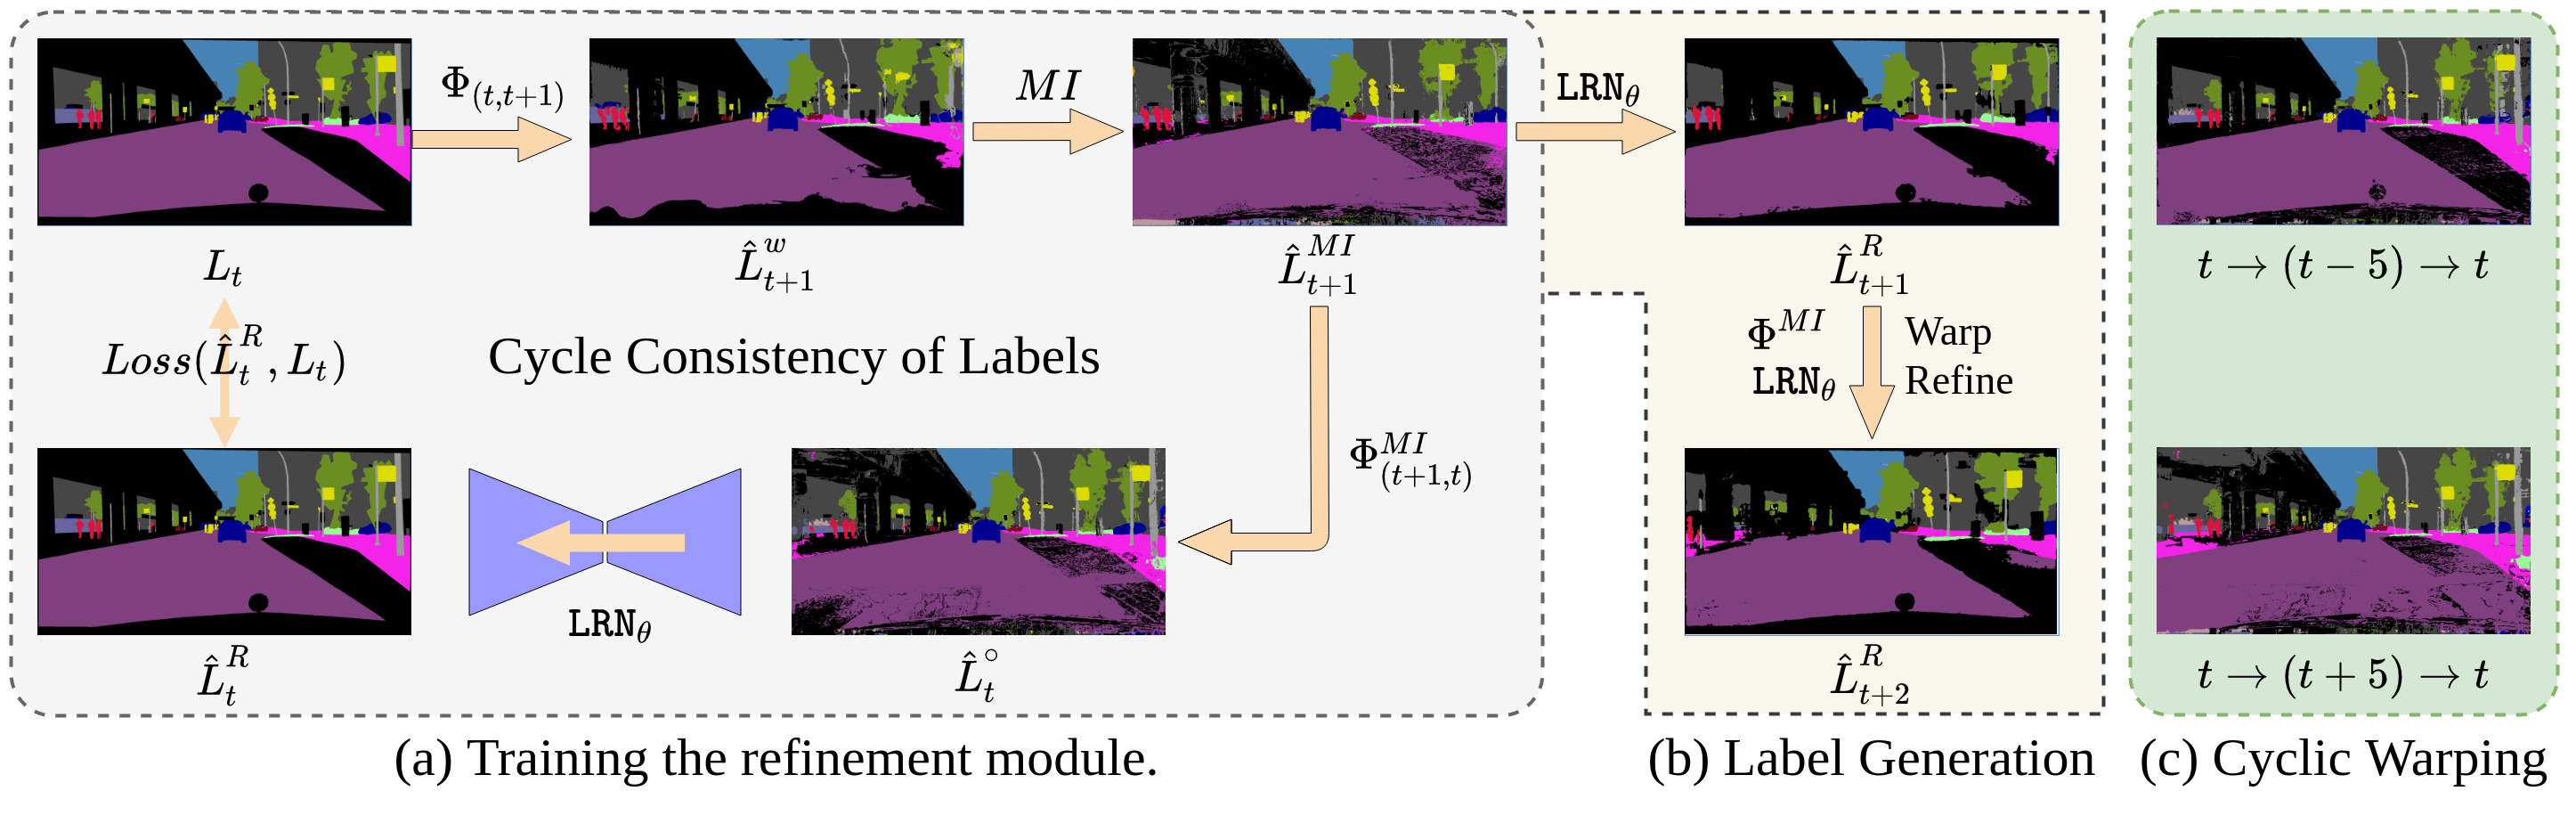
\includegraphics[width=1.0\linewidth]{figures/process_smaller_lr.png}
    \vspace{-2em}
	\caption{\small (a) For training $\texttt{LRN}_\theta$, the cyclic propagated labels $\hat{L}^{\circ}$ are used as input, as given by equation~\eqref{eq-cyclic-process}. (b) While generating labels, the warped post-processed labels $\hat{L}^{MI}$ are given as input to $\texttt{LRN}_\theta$. Iterative application of warping and refining is used to generate sequential labels. (c) The cyclic warped labels are generated for a wider range of cyclic loops to expose $\texttt{LRN}_\theta$ to more warping error while training.}
    \vspace{-1em}
\end{figure}



\subsection{Label Refinement}
\label{subsec-lr}

The warped post-processed labels $\hat{L}^{MI}$ need to be refined as they are still noisy. We do this by training a label refinement network ($\texttt{LRN}_\theta$), parameterized by $\theta$, which takes the pseudo-labels, the warped image, and the clean image, as input, and predicts the refined labels $\hat{L}^{R}$:
\begin{equation}
\label{eq-lrn_inference}
\hat{L}^{R} = \texttt{LRN}_{\theta}(\hat{L}^{MI}, \hat{I}^{w}, I)
\end{equation}

$\texttt{LRN}_\theta$ can be viewed as a denoising network, which takes the noisy samples $\hat{L}^{MI}$ and tries to predict the clean samples $L$. To train any denoising network, we typically need noisy-clean sample pairs. However, for ${t < n \leq t + p}$ we do not contain clean labels $L_{n}$ (as we do not have $D_{Lseq}$). Due to this, we do not have the noisy-clean samples $(L^{MI}, L)$ for training our refinement module. Hence, while using $\mathtt{LRN}_\theta$ is fairly simple, training it is non-trivial.

\textbf{Cycle Consistency of Labels:} With an ideal propagation mechanism, when a label $L_{t}$ is propagated through a cyclic loop in time (say $t$ to $t+1$ and then back to $t$), the resulting cyclic propagated labels (denoted by $\hat{L}^{\circ}_{t}$) should be consistent with initial labels $L_{t}$. Therefore, the inconsistency between $\hat{L}^{\circ}_{t}$ and $L_t$ reveal the modes of failure of the propagation mechanism. We utilize this inconsistency as the supervisory signal to train $\mathtt{LRN}_\theta$.
% \textbf{Cycle Consistency of Labels:} We posit that, with an ideal propagation method, when label $L_{t}$ is propagated through a cyclic loop (for example, $t$ to $t+1$, and then back to $t$), the resulting labels $\hat{L}_{t}$ should be consistent with the $L_{t}$. 
% We utilize this idea for learning how to refine warped labels $\hat{L}^{MI}$. Specifically, we utilize the inconsistency in cyclic propagation of labels as a supervisory signal to train $\mathtt{LRN}_\theta$.
First, we define the cyclic propagated labels $\hat{L}^{\circ}$ for a simple cyclic loop in time:
% If we warp the labels $L_t$ once forward($t$ to $t+1$, generating $\hat{L}^{w}_{t+1}$), and then warp $\hat{L}^{w}_{t+1}$ backwards ($t+1$ to $t$), we generate cyclic propagated labels $\hat{L}^{\circ}$:
% This operation is summarized in the following equations:
\begin{eqnarray}
% \begin{split}
\label{eq-cyclic-process}
    &\Phi_{(t, t+1)}  = f_\theta (I_t, I_{t+1}), \\
    &\hat{I}^{w}_{t+1} = \Phi_{(t, t+1)} (I_{t}) \quad ; \quad \hat{L}^{MI}_{t+1} = \Phi^{MI}_{(t, t+1)} ( \hat{L}^{w}_{t}) \\
    &\Phi_{(t+1, t)}  = f_\theta (\hat{I}^{w}_{t+1}, I_{t}), \\
\label{eq-cyclic}
    &\hat{I}^{\circ}_{t} = \Phi_{(t+1, t)} (\hat{I}^{w}_{t+1}) \quad ; \quad \hat{L}_{t}^{\circ} = \Phi^{MI}_{(t+1, t)} ( \hat{L}^{MI}_{t+1})
% \end{split}
\end{eqnarray}

These cyclic warped labels $\hat{L}_{t}^{\circ}$ contain artifacts created due to the warping process further exacerbated due to the multiple applications of the warping function $\Phi^{MI}$. 
Motivated by the concept of cycle consistency of labels, we utilize the pairs $( \hat{L}_{t}^{\circ},  L_{t})$  as the noisy-clean samples for training $\mathtt{LRN}_\theta$:
\begin{equation}
\label{eq-cyc-train}
% \begin{split}
    \hat{L}^{R} = \texttt{LRN}_\theta(\hat{L}^{\circ}, \hat{I}^{\circ}, I) \quad ; \quad   \theta^{*} = \underset{\theta}{\mathrm{argmin}}\;{ \mathbb{E}(\mathcal{L}(L^{R}, L))},
% \end{split}
\end{equation}
where $\mathcal{L}$ can be any standard loss function such as cross-entropy. In the process of learning to improve consistency between the cyclic warped labels $\hat{L}^{\circ}$ and $L$, $\texttt{LRN}_\theta$ also learns to refine single warped labels $L^{MI}$. It is important to note that cyclic labels, which capture the noise of the warping process, exist because $\Phi_{(t+1, t)} \neq \Phi^{-1}_{(t, t+1)}$.%  (which would otherwise lead to a trivial solution of $\hat{L}_{t}^{\circ} = L_t$). 


Equation~\eqref{eq-cyclic} represents the cyclic labels generated from a single forward and backward step. However, it is possible to perform multiple forward and backward steps, generating multiple $L^{\circ}_{t}$ for each $L_t$. This allows us to capture more diverse artifacts created due to $\Phi^{MI}$. Figure~\ref{fig_method} shows multiple cyclic warped samples for a given label $L_t$.
% We describe the architecture of $\texttt{LRN}_\theta$, inspired from~\cite{pix2pix}, in more details in the supplementary.

Once the refinement module is trained with the cyclic propagated label pairs, we propagate labels by a) warping, b) post-processing, and then finally c) refining with $\mathtt{LRN}_\theta$ to generate refined labels $\hat{L}^R_{t+p}$( refer equation~\eqref{eq-lrn_inference}). This is the complete pipeline of \emph{Warp-Refine Propagation}. At each time step $t+p$, the labels $\hat{L}^R_{t+p}$ undergo propagation to generate $\hat{L}^R_{t+p+1}$.
% This is given by:
% \begin{align}
% \begin{split}
% \label{nvidia_main}
%     \Phi_{(t+p, t+p+1)}  &= f_\theta (I_{t+p}, I_{t+p+1}), \\
%     \hat{L}^{MI}_{t+p+1} &= \Phi^{MI}_{(t+p, t+p+1)} ( \hat{L}^{R}_{t+p}) \\
%     \hat{L}^{R}_{t+p+1} &= LRN(\hat{L}^{MI}_{t+p+1},\hat{I}_{t+p+1}, I{t+p+1} )
% \end{split}
% \end{align}

\subsection{Uncertainty Aware Training}
\label{subsec-alea}

As shown in Figure~\ref{}, the \emph{Warp-Refine Propagation} pipeline generates pseudo-labels of high quality. While these are directly beneficial for training, we note that using labels propagated over a large temporal distance (say $t+10$) can lead to a drop in performance. This is due to the inherent noise in the pseudo-labels. It can be significantly advantageous if we can handle the noise, as psuedo-labels further away from the annotated frame contain novel information. 


%%%%%%%%%%%%%%%%%%%%%%%%%%%%%%%%%%%
%%%%%%%%%%%%%%%%%%%%%%%%%%%%%%%%%%%

% Formally, lets denote labels generated from a given data-generation pipeline as samples of distribution $P_{i}(y|x)$, where as the underlying label distribution is $P(y|x)$.
% % , and labels generated from propagation as samples of distribution $P_{p}(y|x)$. In our case, $D_{L}$ contains samples from $P_{m}(y|x)$, and $D_{\hat{L}seq}$ contains labels from $P_{p}(y|x)$.
% Using model $M_{\theta}(y|x)$, we estimate the distribution the underlying label distribution $P(y|x)$ by maximizing the expected log-likelihood of the model over the given data:
% \begin{equation}
%   \text{Objective} =  \underset{\theta}{\mathrm{argmax}} \big[ \mathbb{E}_{y\sim P(y|x)}\log M_{\theta}(y|x) \big] \sim  \underset{\theta}{\mathrm{argmax}} \sum_{i \in D}{\log M_\theta(y_i|x_i)}
% \end{equation}

% It is important to address the noise in the annotation process, especially in our case, where labels in $D_{Lseq}$ are highly noisy. It is inevitable that a Model which directly maximizes likelihood on $D_L$ and $D_{Lseq}$ under-performs on the test-set as deep networks have a high capacity to memorize noise in the training set[].

% We alleviate the harm caused by noise by modelling the aleatoric uncertainty from the given data. It has been shown that aleatoric uncertainty captures the uncertainty in the data generating process, e.g., inherent measurement noise, and can play a crucial role when training with noisy labels[].
% Specifically, we model $P_m$ and $P_p$ as follows:
% \begin{eqnarray}
%     y &=& \mu(x) + \eta_m \; {\textrm{where }}  y\sim P_m {\textrm{ and }} \eta_m \sim \mathcal{N}(0, \sigma_m^2(x)) \nonumebr \\ 
%     y &=& \mu(x) + \eta_p, \; {\textrm{where }}  y\sim P_p {\textrm{ and }} \eta_p \sim \mathcal{N}(0, \sigma_p^2(x))
% \end{eqnarray}
% Where, $\eta_m$ and $\eta_p$ represent the noise inherent to each annotation process. %Following [], we model $\eta_m$ and $\eta_p$ as additive Gaussian noise with distribution $\mathcal{N}(0, \sigma_m)$ and $\mathcal{N}(0, \sigma_p)$ respectively. 
% We adapt the model parameter $\theta$ specifies the statistics $(\mu^i, \sigma_m^i, \sigma_p^i)$ for each pixel $i$ in a given image $x$. The optimization objective can now be written as: 
% \begin{align}
% \begin{split}
%     %(\mu^i, \sigma_m^i, \sigma_p^i) &= M_{\theta}(x^i) \\
%     l_m^i |\theta \sim \mathcal{N}(\mu^i, \sigma_m^i) \quad &; \quad \hat{p^i_m} = \softmax(\hat{l^i_m}) \\
%     l_p^i |\theta \sim \mathcal{N}(\mu^i, \sigma_p^i) \quad &; \quad \hat{p^i_p} = \softmax(\hat{l^i_p}) \\
% \end{split}
% \end{align}
% \begin{equation}
%     \text{Objective} =  \underset{\theta}{\mathrm{argmax}} \Bigg[ \sum_{m \in D_L}{\log E_{\hat{l^i_m} \sim  \mathcal{N}(\mu^i, \sigma^i_m)}(\hat{p^i_m})} + \sum_{p \in D_{Lseq}}{\log E_{\hat{l^i_p} \sim  \mathcal{N}(\mu^i, \sigma^i_p)}(\hat{p^i_p})} \Bigg]
% \end{equation}

% \let\clearpage\relax
% 
%%%%%%%%%%%%%%%%%%%
%%% SVHN RESULTS
%%%%%%%%%%%%%%%%%%%
\begin{figure}[t]
\begin{center}\small
\setlength{\tabcolsep}{3pt}
		\subfigure[Mean IOU of various propagation methods.]
		{
			\begin{minipage}{0.58\textwidth}
				\label{fig:input-model}
				% \centering
				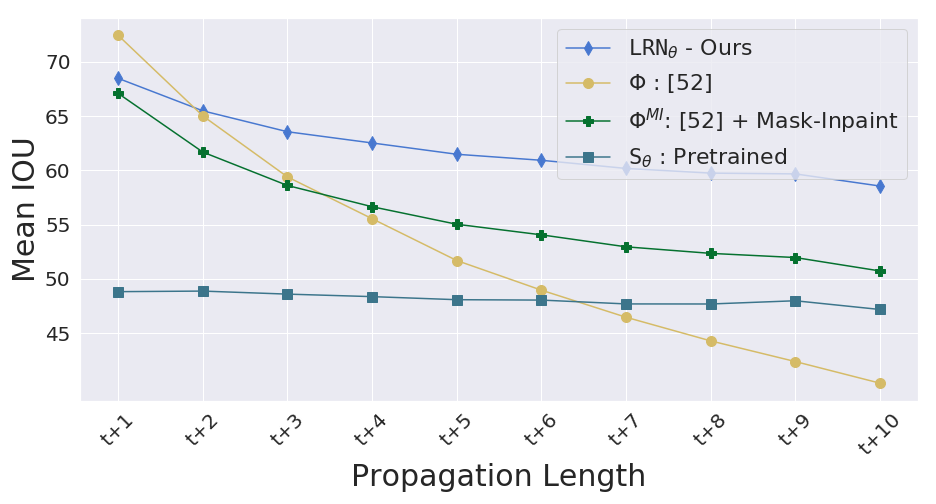
\includegraphics[width=1.0\linewidth]{figures/miou_apollo.png}
				\hfill
				\vfill
			\end{minipage}
		}
% \hspace{-1em}
% \vtop{
% \vspace{-1em}
\hfill
% \hbox{
% 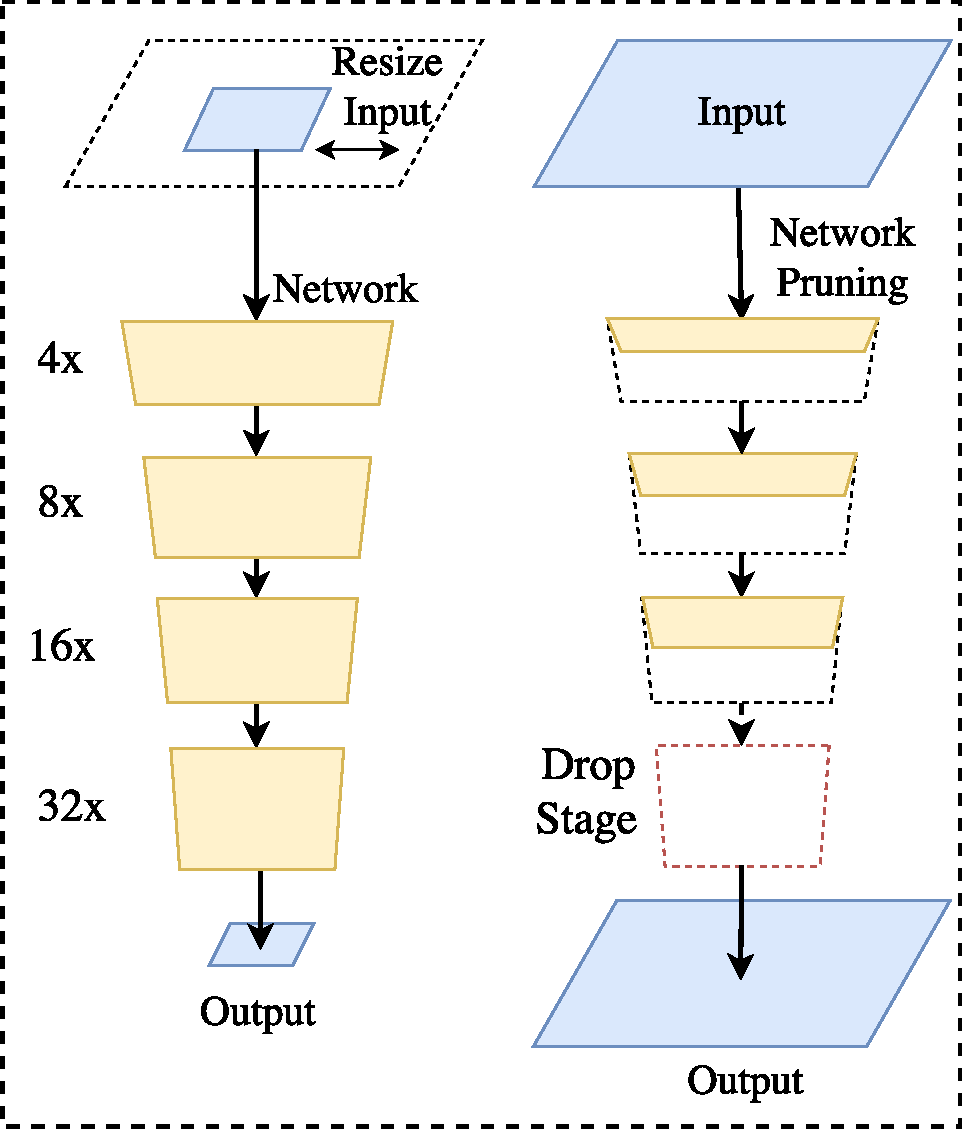
\includegraphics[width=0.6\textwidth]{figures/input_model.pdf}
		\subfigure[Qualitative Example]{
            \begin{minipage}{0.35\textwidth}
                \centering
				\label{fig:input-model}
				% \centering
				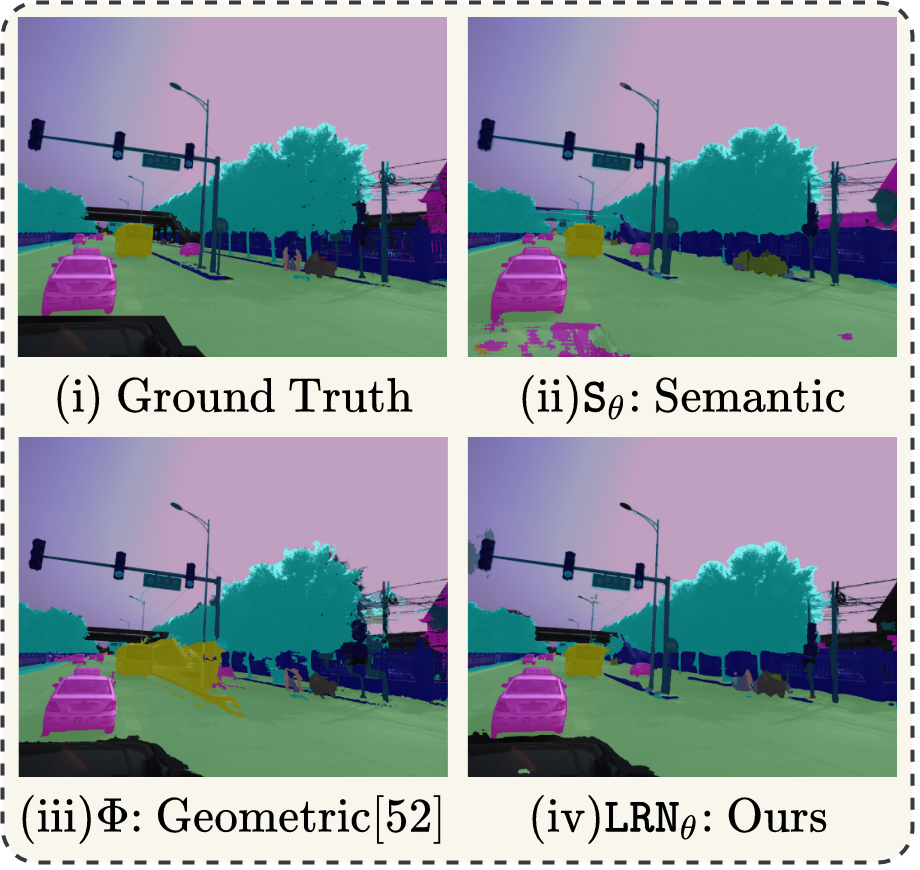
\includegraphics[width=1.0\linewidth]{figures/apollo_vis.png}
\end{minipage}
% }}%
}
\end{center}
\vspace{-1em}
\caption{\small \emph{(a)} We \textit{quantitatively} show that our method is significantly better than previous \textit{state-of-the-art} method. \emph{(b)} \cite{nvidia_cvpr19}, which uses geometric information is suspectible to poor warping, on the other hand generating pseudo-labels from semantic predictions (via network $\mathtt{S}_\theta$ poorly labels rare classes. Our method combines geometric and semantic information together, generating cleaner labels.}
\label{table:svhn}

		\vspace{-1em}
\end{figure}

% where $p_i$ represents the probability vector. 
% Due to the lack of analytical solution for $E(p_i)$, we approximate the object by monte carlo integration as described in []. This entails drawing $t$ samples from the distribution  $\mathcal{N}(\mu^i, \sigma^i)$ and calculating the empirical mean probability vector $p^i$ at each pixel. As both the data generation process noises $\eta_m$ and $\eta_p$ are modelled as zero-mean Gaussian noises, $\softmax(\mu^i)$ models the underlying distribution $P(y|x)$. Hence at test-time, our predictions for a given image is simply $\mu^i$ for each pixel $i$ in the image.

% In practice, this objective simply means that we model separate aleatoric uncertainty for each of label dataset $D_L$ and $D_{Lseq}$. We add a two small heads to the given segmentation models to predict $\sigma_m$ and $\sigma_p$, and while calculating the loss, if the label is from $D_L$ we utilize the $\sigma_m$ , if the label is from $D_{Lseq}$ we utilize $\sigma_p$. In section~\ref{} we show the benefits of this approach over previous methods, as well as over modelling a single aleatoric uncertainty for the combined dataset $D_L$ and $D_{Lseq}$.

% % FOR Experiements
% \subsection{Different Narrative}

%%%%%%%%%%%%%%%%%%%%%%%%%%%%%%%%%%%%%%%%%%
%%%%%%%%%%%%%%%%%%%%%%%%%%%%%%%%%%%%%%%%%%%

Formally, let us denote labels generated from a given noisy data-generation process $\delta$ as samples of distribution $P_{\delta}(y|x)$, whereas the underlying label distribution is $P(y|x)$.
% , and labels generated from propagation as samples of distribution $P_{p}(y|x)$. In our case, $D_{L}$ contains samples from $P_{m}(y|x)$, and $D_{\hat{L}seq}$ contains labels from $P_{p}(y|x)$.
Typically, using model $M_{\theta}(y|x)$ parameterized by $\theta$, we estimate the underlying label distribution $P(y|x)$ by maximizing the expected log-likelihood of the model over the given data:
\begin{equation}
   \theta^{*} =  \underset{\theta}{\mathrm{argmax}} \big[ \mathbb{E}_{y\sim P(y|x)}\log M_{\theta}(y|x) \big] \sim  \underset{\theta}{\mathrm{argmax}} \sum_{i \in D}{\log M_\theta(y_i|x_i)},
\end{equation}
where $\theta^{*}$ represents the optimal parameters for $M_\theta$. Since we contain noisy samples from $P_{\delta}$, our model is biased to model $P_{\delta}$, rather than $P$. To address the distributional shift between $P_\delta$ and $P$ we modify the objective of our optimization. 
Let us consider the relation between noisy labels and clean labels as $P(y_\delta|x,y)$, where $y_\delta$ represents the noisy sample for a given $x$. Since we want $M_\theta$ to model the underlying label distribution $P$, we can rewrite our estimate $P_\theta$ for noisy labels $y_\delta$, and the corresponding objective as:
% \begin{eqnarray}
% \begin{split}
%     P(y_\delta|x) &= \sum_{y'}P(y_\delta | x, y')P(y=y'|x), \\  
%     P_\theta(y_\delta|x) &= \sum_{y'}(P(y_\delta | x, y')+\Delta(y_\delta | x, y'))M_\theta(y=y'|x) \label{eq:noisy distribution}
% \end{split}
% \end{eqnarray}
\begin{equation}
    P(y_\delta|x) = \sum_{y'}P(y_\delta | x, y')P(y=y'|x) \quad ; \quad P_\theta(y_\delta|x) = \sum_{y'}(P(y_\delta | x, y'))M_\theta(y=y'|x)
\label{eq:noisy distribution}
\end{equation}
\begin{equation}
%   \text{Objective} \sim  \underset{\theta}{\mathrm{argmax}} \big[ \sum_{y_\delta \sim P_\delta}{\log \sum_{y'}P(y_\delta|x_i, y')M_\theta(y'| x_i)} \big]
   \theta^{*} \sim  \underset{\theta}{\mathrm{argmax}} \big[ \sum_{y_\delta \sim P_\delta}{\log P_\theta(y_\delta | x)} \big]
   \label{eq_new_object}
\end{equation}

\begin{theorem}
\label{thm:dtv bound}
Let $\epsilon = 1-\min_{y'}P(y_\delta=y' | x, y')$.
If $\epsilon < 0.5$, then the following inequality holds for the distributions $P(y_\delta|x)$ and $P_\theta(y_\delta|x) $ defined in Eq.\eqref{eq:noisy distribution}.
\begin{align}
    d_{TV}(P(y|x), M_\theta(y|x)) \leq 
    \frac{1}{1-2\epsilon}
    \left(\sqrt{2KL[P(y_\delta|x)|P_\theta(y_\delta|x)]}
    + \gamma  \right).\label{eq:dtv_bound}
\end{align}
where $d_{TV}(p(y),q(y))$ is the total variation distance and $KL[p(y)|q(y)]$ is the Kullback-Leibler divergence.
% where $\gamma = \frac{1}{2}\sum_{\hat{y}}|\sum_y \Delta(\hat y|y,x)M_\theta(y|x)|$, $d_{TV}(p(y),q(y)) = \frac{1}{2}\sum_y |p(y)-q(y)|$ is a total variation distance and $KL[p(y)|q(y)] = \sum_y p(y)\log\frac{p(y)}{q(y)}$ is a Kullback-Leibler divergence.
\end{theorem}

% Need to update theorem to be without reference to \Delta. 
Therefore, our objective~\eqref{eq_new_object} which minimizes the KL-divergence between $P(y_\delta|x)$ and $P_\theta(y_\delta|x)$, lowers the total variation distance between  $P(y|x)$ and $M_\theta(y|x)$ as well. The proof is provided in the supplementary.

% When $\Delta(y_\delta | x, y')=0$, 
% Theorem 1 implies that we can completely minimize the total variation distance between the true label distribution $P(y|x)$ and model distribution $M_\theta(y|x)$ through the learning of the noisy label distribution $P(y_\delta|x)$ 
% by using the model $P_\theta(y_\delta|x)$ 
% as long as $\min_{y'}P(y_\delta=y' | x, y') > 0.5$.
% On the other hand, when $\Delta(y_\delta | x, y')$ is nonzero, we can minimize the total variation distance only up to the constant $\frac{\gamma}{1-2\epsilon}$.

%In the supplementary, we prove that minimizing the KL-divergence between $P(y_\delta|x)$ and $P_\theta(y_\delta|x)$ minimizes the total variation distance $d_{TV}$ between  $P(y|x)$ and $M_\theta(y|x)$. 
% Formally: 
% \begin{equation}
%     d_{TV} (P(y|x),M(y|x)) \leq KL_D(P(y_\delta|x),P_\theta(y_\delta|x))
% \end{equation}
% Note that our proof is for a known relation $P(y_\delta |x, y )$, in practice, we use only an estimate $\hat{P}(y_\delta |x, y)$. 
Note that our formulation is independent of the labelling process $\delta$, and hence can be used for multiple labelling processes $\delta_j; j \in \mathbb{N}$.
% Let us denote $P_\theta(y_{\delta_0} | x) = M_\theta(y|x)$ by assuming the manual annotation is also a kind of noisy labeling process.
Now, we model $P_\delta$ and as a noisy version of $P$. Taking inspiration from~\cite{gal_main}, 
we represent $P_\theta(y_{\delta_j} | x)$ as:
%for a given labelling process $\delta_j$ we model the relation between clean and noisy labels as:
\begin{align}
    P_\theta(y_{\delta_j} = k | x) &= E_{a^{i}_{j,k} \sim \mathcal{N}(\mu^i_k(x), \sigma_{\delta_j}^i(x))}[\softmax(a^{i}_{j,k})]
\end{align}
where $\softmax(a_k) = \exp(a_k)/\sum_{k'}\exp(a_{k'})$ is the softmax function.
% \begin{equation}
%     y_{\delta_j} = y + \eta_{\delta_j} \; {\textrm{where }}  y_{\delta_j} \sim P_{\delta_j}, y \sim P(y|x){\textrm{ and }} \eta_{\delta_j} \sim \mathcal{N}(0, \sigma_{\delta_j}^2(x))
% \end{equation}
% Where, $\eta_{\delta_j}$ represent the noise inherent to each labelling process $\delta_j$ (the relation $P(y_{\delta_j}| x, y)$ is modelled by the additive Gaussian noise $\eta_{\delta_j}$).% (hence P()). %Following [], we model $\eta_m$ and $\eta_p$ as additive Gaussian noise with distribution $\mathcal{N}(0, \sigma_m)$ and $\mathcal{N}(0, \sigma_p)$ respectively. 
We adapt the model parameter $\theta$ to model the statistics $(\mu^i(x), \sigma_{\delta_0}^i(x),\sigma_{\delta_1}^i(x), .. )$ for each pixel $i$ in a given image $x$. The optimization objective can now be written as: 
% \begin{align}
% \begin{split}
%     %(\mu^i, \sigma_m^i, \sigma_p^i) &= M_{\theta}(x^i) \\
%     l_{\delta_j}^i |\theta \sim \mathcal{N}(\mu^i, \sigma_{\delta_j}^i) \quad &; \quad \hat{p^i_{\delta_j}} = \softmax(\hat{l^i_{\delta_j}}) \\
% \end{split}
% \end{align}
\begin{equation}
    % \text{Objective} =  \underset{\theta}{\mathrm{argmax}} \Bigg[ \sum_{\delta_j}{\sum_{i \in D_{{\delta_j}}}{\log \mathbb{E}_{\hat{l^i_{\delta_j}} \sim  \mathcal{N}(\mu^i, \sigma^i_{\delta_j})}(\hat{p^i_{\delta_j}})}} \Bigg]
    \theta^{*} =  \underset{\theta}{\mathrm{argmax}} \Bigg[ \sum_{j}{\sum_{i \in D_{{\delta_j}}}{\log P_\theta(y_{\delta_j} | x)}} \Bigg]
\end{equation}

\let\clearpage\relax

%%%%%%%%%%%%%%%%%%%
%%% SVHN RESULTS
%%%%%%%%%%%%%%%%%%%
\begin{figure}[t]
\begin{center}\small
\setlength{\tabcolsep}{3pt}
		\subfigure[Mean IOU of various propagation methods.]
		{
			\begin{minipage}{0.58\textwidth}
				\label{fig:input-model}
				% \centering
				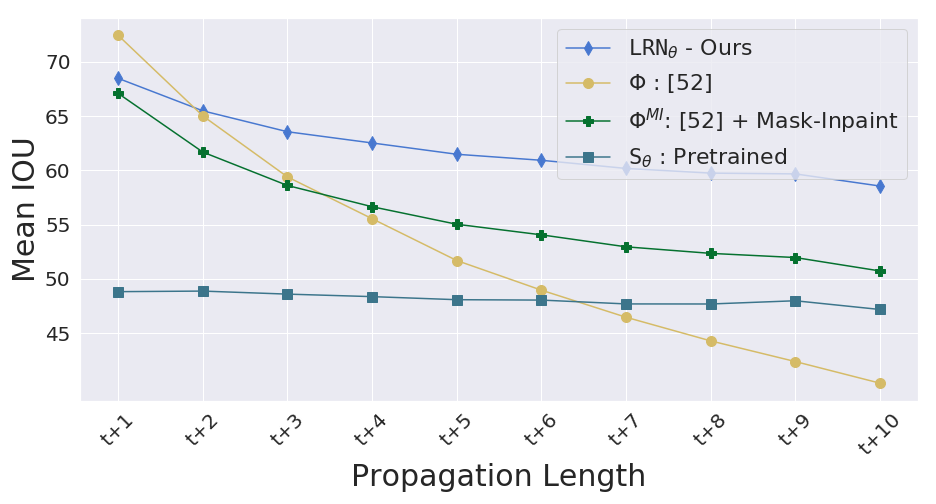
\includegraphics[width=1.0\linewidth]{figures/miou_apollo.png}
				\hfill
				\vfill
			\end{minipage}
		}
% \hspace{-1em}
% \vtop{
% \vspace{-1em}
\hfill
% \hbox{
% 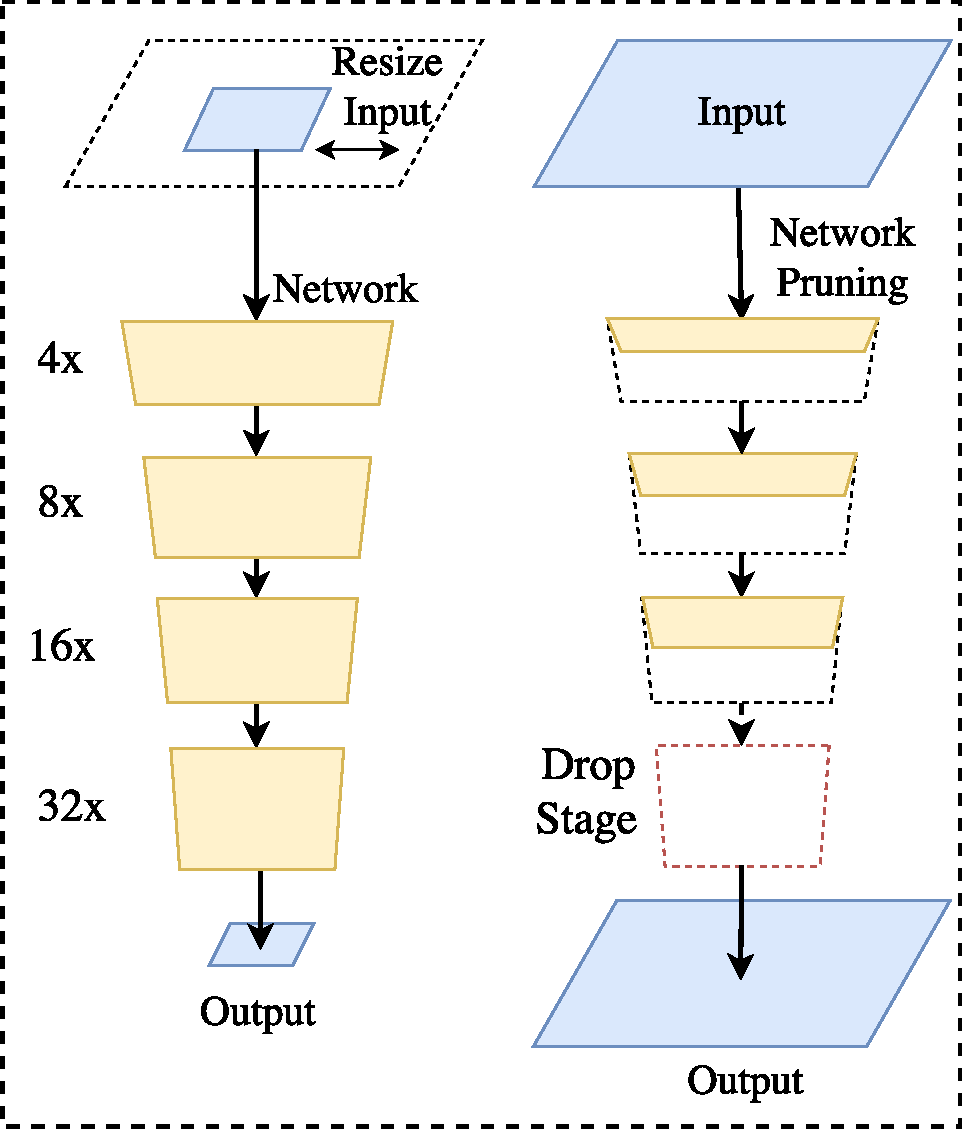
\includegraphics[width=0.6\textwidth]{figures/input_model.pdf}
		\subfigure[Qualitative Example]{
            \begin{minipage}{0.35\textwidth}
                \centering
				\label{fig:input-model}
				% \centering
				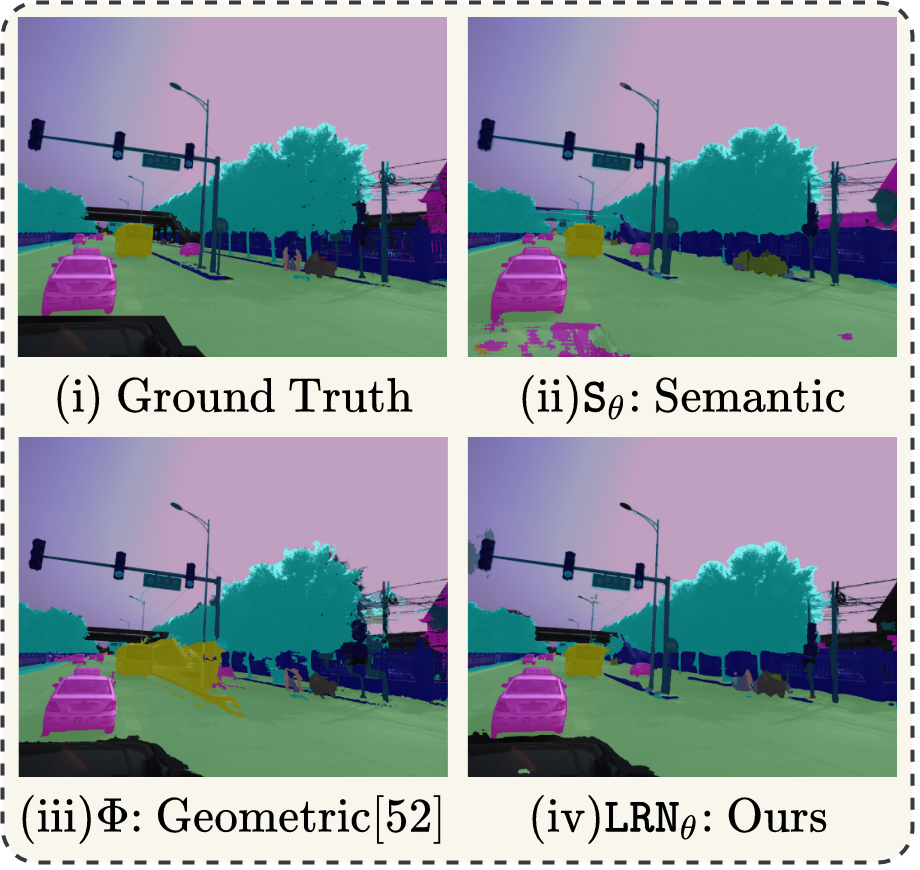
\includegraphics[width=1.0\linewidth]{figures/apollo_vis.png}
\end{minipage}
% }}%
}
\end{center}
\vspace{-1em}
\caption{\small \emph{(a)} We \textit{quantitatively} show that our method is significantly better than previous \textit{state-of-the-art} method. \emph{(b)} \cite{nvidia_cvpr19}, which uses geometric information is suspectible to poor warping, on the other hand generating pseudo-labels from semantic predictions (via network $\mathtt{S}_\theta$ poorly labels rare classes. Our method combines geometric and semantic information together, generating cleaner labels.}
\label{table:svhn}

		\vspace{-1em}
\end{figure}

%where $p^i$ represents the probability vector. 
Due to the lack of analytical solution for $ P_\theta(y_{\delta_j} | x)$, %  $\mathbb{E}(p^i)$, 
we approximate the objective by Monte Carlo integration as described in~\cite{gal_main}. %This entails drawing $t$ samples from the distribution  $\mathcal{N}(\mu^i, \sigma^i)$ and calculating the empirical mean probability vector $p^i$ at each pixel. 
% As all the data generation process noises $\eta_{\delta_j}$ are modelled as zero-mean Gaussian noises, 
As $\softmax(\mu^i)$ models the underlying distribution $P(y|x)$, at test-time, our predictions for a given image is simply $\mu^i$ for each pixel $i$ in the image.

In practice, this objective translates to modelling separate aleatoric uncertainty components for each of the noisy labelling processes $\delta_j$. The aleatoric uncertainty is modelled by adding a small two-layer head to the given segmentation models to predict $\sigma_{\delta_j}$. In Section~\ref{section-exp}, we show the benefits of this approach over modelling a single aleatoric uncertainty for the combined dataset.

\textbf{Using Pseudo Labels}: We also utilize pseudo-semantic labelling~\cite{taskonomy2018, pseudo_nips_1} for data points where label propagation is not possible. For Cityscapes~\cite{cs_dataset}, we use predictions from a model $S_\theta$ trained utilizing only the labels $D_L$, to create dataset $D_{\hat{L}ps}$ (specifically, labels for the \texttt{train\_extra} subset of Cityscapes). As our training procedure is agnostic to the label generation process, we can use the different labels by simply modelling a separate uncertainty parameter $\sigma_{\delta_j}$ for each of them. 
% $D_L$, $D_{\hat{Lseq}}$ and $D_{\hat{L}ps}$ to train our final model by simply modelling the three noise processes $\eta_L$, $\eta_{\hat{Lseq}}$ and $\eta_{\hat{L}ps}$ respectively.

% \begin{equation}
%     log E_{\hat{l_i} \sim  \mathcal{N}(u_i, \sigma_i)}(\hat{p_i}) \sim log(\frac{1}{T}\sum_{t}{\text{soft}_{\text{max}} (u_i + \epsilon_t * \sigma_i)}
% \end{equation}
% The problem with [below para] is that while our objective/modelling changed, there is no guarentee that is what will happen inside. Also it makes it hard to get to why a sigma for clean labels. However, if we start from Aleatoric, and then highlight this feature in discussions, we can make the link to generic noisy augmentation processes. 


% To address this mismatch between the objective and the optimization process, we change our optimization process. Specifically, we introduce a parameterized model $M_\beta$ to model the distribution $P(y_\delta|x, y)$ where $y \sim P(y|x)$ and $y_\delta \sim P_\delta(y|x)$. This model tries to estimate the conditional distribution of the noisy labels, given the clean labels, and corresponding image $x$. Hence, our learning objective becomes:

% Modelling the noise $\eta$ is a parameterized modelling of $P(y_\delta|x,y)$. It can be seen as a separate model $M_\beta$, with the final objective:
% \begin{equation}
%     M_{(\theta, \beta)} \sim  \underset{(\theta, \beta)}{\mathrm{argmax}} \big[ \sum_{y_m \in D_L}{\log M_\theta(y_m|x_m)} + \sum_{y_{n\delta} \in D_{Lseq}}{\log (M_\beta(y_{n\delta}|x_n,y_n)  M_\theta(y_n|x_n)) \big]}
% \end{equation}





\section{Experiments}
\label{section-exp}


\let\clearpage\relax


% \begin{table}
% 	\begin{minipage}{0.5\linewidth}
% 		\caption{Student Database}
% 		\label{table:student}
% 		\centering

% \begin{tabular}[t]{llc}
% %%%%%% Title row starts here
% % Temporary header Graph would be better! TBD
% \toprule
% \multicolumn{2}{l}{} & mIOU \\
% \midrule
% \multicolumn{2}{l}{Baseline} & 75.79 \\
% \multicolumn{2}{l}{Baseline + SDC} & 76.37 \\
% \multicolumn{2}{l}{Baseline + LID} & 76.37 \\
% \bottomrule
% \end{tabular}
% 	\end{minipage}\hfill
% 	\begin{minipage}{0.45\linewidth}
% 		\centering
% 		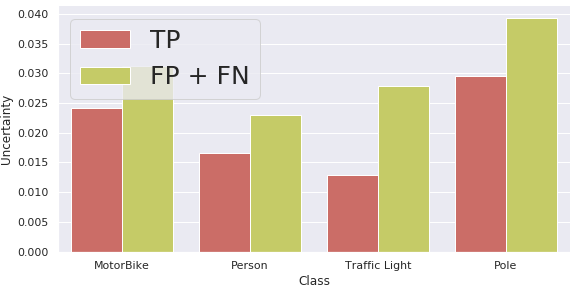
\includegraphics[width=1.0\linewidth]{figures/uncertainty.png}
% 		\captionof{figure}{2-D scatterplot of the Student Database}
% 		\label{ }
% 	\end{minipage}
% \end{table}
\begin{figure}\CenterFloatBoxes
\begin{floatrow}
\ffigbox[1.0\linewidth][]
{%
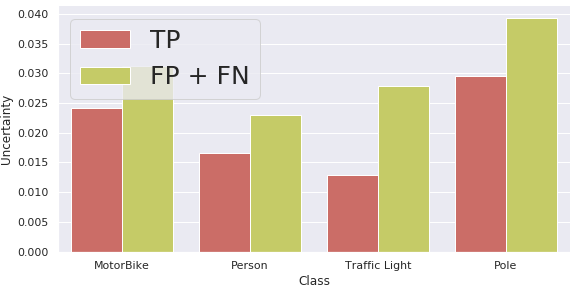
\includegraphics[height=0.4\linewidth]{figures/uncertainty.png}}
{%
\vspace{-0.3em}%
\caption{ Precision vs Recall plot showing uncertainty effectively captures noise in label generation.}\label{fig: figure-label}}
\killfloatstyle\ttabbox[\Xhsize]
{%
\begin{tabular}[b]{llc}
%%%%%% Title row starts here
% Temporary header Graph would be better! TBD
\toprule
\multicolumn{2}{l}{} & mIOU \\
\midrule
\multicolumn{2}{l}{Baseline} & 77.66 \\
\multicolumn{2}{l}{Baseline  + \cite{nvidia_cvpr19} ($\pm 3$)}+ RLL  & 77.24 \\
\multicolumn{2}{l}{Baseline + Ours($\pm 3$)}+ RLL  & 77.50 \\
\bottomrule
\end{tabular}%
}%
{\caption{ Addding a single propagated frame, and relaxed label loss (RLL)~\cite{nvidia_cvpr19} is ineffective.}\label{tab: table-label}}%
\end{floatrow}

% \caption{\small \emph{Left:} The sequence error for SVHN multi-digit recognition
% on crops of $64\times 64$ pixels (64px), and inflated crops of $128 \times 128$
% (128px) which include more background. \textsuperscript{*}The best reported
% result from \cite{Ba14} uses model averagin}
% % }}%
\vspace{-1em}
\end{figure}

% \begin{figure}
% \begin{floatrow}
% \capbtabbox{%
% \centering%
% \begin{tabular}[t]{llc}
% %%%%%% Title row starts here
% % Temporary header Graph would be better! TBD
% \toprule
% \multicolumn{2}{l}{} & mIOU \\
% \midrule
% \multicolumn{2}{l}{Baseline} & 75.79 \\
% \multicolumn{2}{l}{Baseline + SDC} & 76.37 \\
% \multicolumn{2}{l}{Baseline + LID} & 76.37 \\
% \bottomrule
% \end{tabular}
% }{%
%   \caption{This is the great table of asgard}%
% }%
% \ffigbox{%
% \centering%
% 				\label{fig:input-model}
% 				% \centering
% 				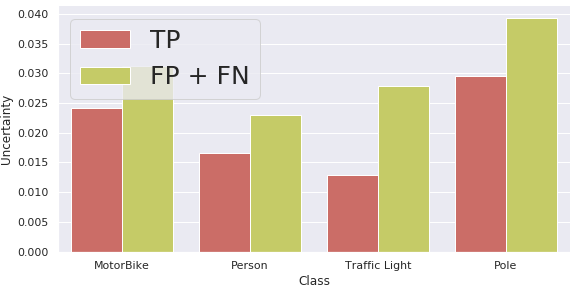
\includegraphics[width=0.5\linewidth]{figures/uncertainty.png}%
% }{%
%   \caption{A figure from asgard}%
% }%
% \end{floatrow}
% \end{figure}



% \begin{figure}[t]
% \begin{center}% \small
% % \setlength{\tabcolsep}{3pt}

% \label{table:svhn}
% 		\subfigure[b]{
% \begin{minipage}{0.45\textwidth}
% \centering
% \begin{tabular}[t]{llc}
% %%%%%% Title row starts here
% \\
% % Temporary header Graph would be better! TBD
% \toprule
% \multicolumn{2}{l}{} & mIOU \\
% \midrule
% \multicolumn{2}{l}{Baseline} & 75.79 \\
% \multicolumn{2}{l}{Baseline + SDC} & 76.37 \\
% \multicolumn{2}{l}{Baseline + LID} & 76.37 \\
% \bottomrule
% \end{tabular}
% \end{minipage}
% % }}%
% \caption{Corrected Evalutation of previous work\cite{nvidia_cvpr19}}
% }
% % \qquad\qquad \qquad\qquad
% % \hspace{2em}
% % \vtop{
% % \hfill
% % \hbox{
% % 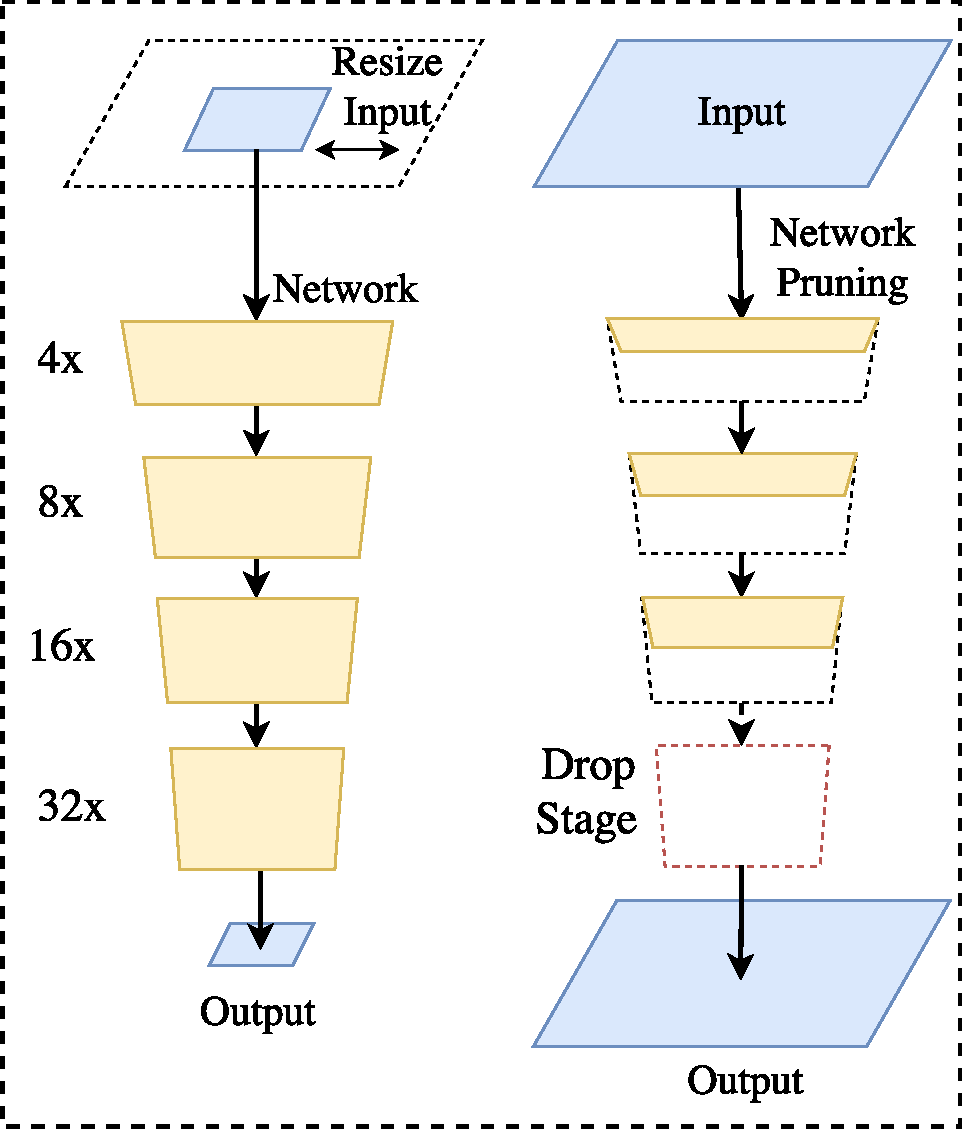
\includegraphics[width=0.6\textwidth]{figures/input_model.pdf}
% 		\subfigure[b]{
% \begin{minipage}{0.30\textwidth}
% \centering
% 				\label{fig:input-model}
% 				% \centering
% 				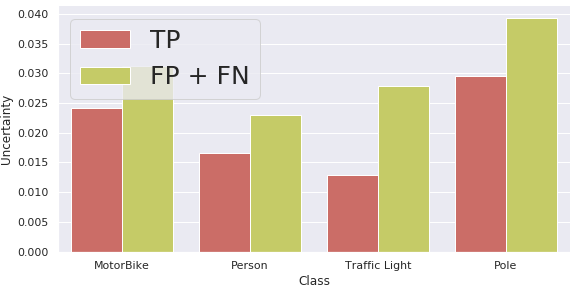
\includegraphics[width=1.0\linewidth]{figures/uncertainty.png}
% \end{minipage}
% \caption{Precision-Recall Curve}
% }

% \caption{\small \emph{Left:} The sequence error for SVHN multi-digit recognition
% on crops of $64\times 64$ pixels (64px), and inflated crops of $128 \times 128$
% (128px) which include more background. \textsuperscript{*}The best reported
% result from \cite{Ba14} uses model averagin}
% % }}%
% \end{center}
% 		\vspace{-2.0em}
% \end{figure}


\let\clearpage\relax
\begin{table}[t]
    \centering
    \caption{ We show the benefit of training with our pseudo-labels. We also show the benefit of modelling label uncertainty. In the above table,  $D_{\hat{L}seq}$ contains propagated labels and $D_{\hat{L}ps}$ contains pseudo-semantic labels (refer Section~\ref{subsec-alea}).
    }\label{tab_main_ablation}
    \begin{tabular}{llccc}
\toprule
\multicolumn{2}{c}{Dataset}& Cross Entropy & Aleatoric Uncertainty\cite{gal_main} & Ours: UAT \\
\midrule
\multicolumn{2}{l}{$D_L$} & 77.62 & 77.69 & - \\
\multicolumn{2}{l}{$D_L + D_{\hat{L}seq}$ }& 77.82 & 77.83 & 78.11 \\
\midrule
\multicolumn{2}{c}{$D_L + D_{\hat{L}seq} + D_{\hat{L}ps}$} & 78.45  & 78.52 & \textbf{78.58} \\
\bottomrule
    \end{tabular}
\end{table}
%Now, we present quantitative and qualitative evaluation of our proposed method. We break this section into two major parts: Evaluation of the propagation method, Evaluation of learning with propagated labels. Our experiments are performend on two widely adopted semantic segmentation datasets, Cityscapes and Apolloscape.

\subsection{Implementation Details}
For training the label refinement network $\mathtt{LRN}_\theta$, we utilize the dual-task loss~\cite{gated_iccv2019}.
For training semantic segmentation networks on manually annotated and generated labels we follow the training regime outlined by~\cite{nvidia_cvpr19} as our baseline. However, we do not use Relaxed Label Loss~\cite{nvidia_cvpr19} (cf. Section~\ref{subsec-lp_train}), and train all models for $220$ epochs. The network architecture is based on DeepLabV3+~\cite{deep_v3} with a ResNeXt~\cite{resnext} backbone for ablations, and WideResNet38~\cite{wider_res38} for the test set submissions.
The architecture and other training details are explained in the supplementary.

\textbf{Dataset Details}: The ApolloScape dataset~\cite{as_dataset} contains 143,906 annotated images. To make our study feasible, we first create train and validation subsets of sizes 40,100 and 6,113 respectively. We further divide the train-subset into $D_I$ and $D_{Iseq}$ containing 2,005 and 40,100 images respectively by creating continuous partitions of 21 frames each (more details are outlined in the supplementary). As ApolloScape has annotation for all frames, we have the ground truth label set $D_{Lseq}$ containing the clean annotations. We evaluate models trained with clean and propagated labels on the untouched validation subset. The Cityscapes dataset~\cite{cs_dataset} consists of 5,000 annotated images, split as the train ($D_{I}$), validation and test set with 2,975, 500, and 1,525 images, respectively. Further, a subset with sequential images containing no annotation $D_{Iseq}$, and a subset $D_{Ips}$ containing coarse annotation is also provided. Note that we \textit{do not} use the coarse labels and instead utilize pseudo-labelling for $D_{\hat{L}ps}$. % Models trained with clean and generated labels are evaluated on the val and test partitions. 


\subsection{Evaluating Label Propagation}
\label{subsec-lp_eval}
We quantitatively establish that our method is able to propagate labels with significantly lesser noise than existing methods. 
%Using the clean annotation $D_{Lseq}$ in Apolloscape we evaluate different the propagation methods. 
In the ApolloScape dataset, from the manually annotated labels in $D_L$, we generate the approximated labels $D_{\hat{L}seq}$ for each propagation technique, and evaluate it against the given annotated labels $D_{Lseq}$.

Figure~\ref{} show the mean Intersection over Union (mIoU) of different propagation methods at each propagation length. 
% This is evaluated on the sequences adjacent to the training set itself, as label propagation is also conducted on those sequences only. 
We compare against the previous state-of-the-art~\cite{nvidia_cvpr19}, as well as predictions from a segmentation model $\mathtt{S}_\theta$ trained on $D_L$ only. Our label propagation method surpasses the other methods, and as shown, \cite{nvidia_cvpr19} quickly start performing even worse than $\mathtt{S}_\theta$. 
% We also present some qualitative results in Figure~\ref{} comparing nvidia etal with warp-refine propagation on Cityscapes.


\subsection{Learning with Generated Labels}
\label{subsec-lp_train}

 We evaluate the improvement in semantic segmentation by training a model on the generated labels. We report the mean value of each metric over three different runs.%  Hence, our baseline model is  only labels $D_L$.
%(i.e., for Cityscapes we do not use Coarse Labels, or pretraining on mapillary). 

First, we present results countering the claims of the previous work~\cite{nvidia_cvpr19}. Specifically, we find~\cite{nvidia_cvpr19} to be ineffective in improving semantic segmentation. The baseline reported in ~\cite{nvidia_cvpr19} is trained for one-third the iterations with a suboptimal learning rate. By equalizing the number of training iterations, and increasing learning rate, we find that the baseline is able to match the proposed models from~\cite{nvidia_cvpr19}.~\footnote{We use the code provided by the authors at \url{https://github.com/NVIDIA/semantic-segmentation}. A similar trend is observed even when using coarse labels, and Mapillary Vistas pretraining and is reported in the supplementary.}


\let\clearpage\relax

\begin{table}[t]
  \caption{\small \textit{State-of-the-art} methods on the Cityscapes dataset (test partition)}
  \label{gta5-cts}
  \centering
  \scalebox{0.582}{
  \begin{tabular}{cccccccccccccccccccccc}
    \toprule
   % \multicolumn{22}{c}{\textbf{GTA5 $\rightarrow $ Cityscapes}}                   \\
    % \cmidrule(r){1-2}
    % Name     & Description     & Size ($\mu$m) \\
     \ & \rotatebox{90}{road}& \rotatebox{90}{sidewalk}& \rotatebox{90}{building} &\rotatebox{90}{wall} &\rotatebox{90}{fence} &\rotatebox{90}{pole} &\rotatebox{90}{light} & \rotatebox{90}{sign} &\rotatebox{90}{vege.} &\rotatebox{90}{terrain} &\rotatebox{90}{sky} &\rotatebox{90}{person} &\rotatebox{90}{rider} &\rotatebox{90}{car} &\rotatebox{90}{truck} &\rotatebox{90}{bus} &\rotatebox{90}{train} &\rotatebox{90}{motor} &\rotatebox{90}{bike} &mIoU \\%&gain \\
    \midrule
				% DepthSeg \cite{Kong2018depthseg}  &  98.5  &  85.4  &  92.5  &  54.4  &  60.9  &  60.2  &  72.3   & 76.8   & 93.1   & 71.6   & 94.8  &  85.2  &  68.9   & 95.7  &  70.1  &  86.5  &  75.5   & 68.3   & 75.5   & 78.2 \\
				% PSPNet  \cite{Zhao2017pspnet}       &  98.6 & 86.2 & 92.9 & 50.8 & 58.8 & 64.0 & 75.6 &  79.0 & 93.4 & 72.3 & 95.4 & 86.5 & 71.3 & 95.9 & 68.2 & 79.5 & 73.8 & 69.5 & 77.2 & 78.4        \\
				% AAF  \cite{Ke2018AAF} &  98.5  & 85.6  & 93.0  & 53.8  & 58.9  & 65.9  & 75.0  & 78.4  & 93.7  & 72.4  & 95.6  & 86.4 &  70.5 &  95.9  & 73.9 &  82.7 &  76.9 &  68.7  & 76.4  & 79.1 \\
				% PanoDeepLab \cite{Cheng2019DeepLabPano} &  98.7 & 87.2 &  93.6  & 57.7  & 60.8  & 70.8 &  78.0 &  81.2 &  93.8 &  74.1 &  95.7 &  88.2 &  76.4  & 96.0  & 55.3  & 75.1 &  79.6 &  72.1 &  74.0  &     $79.4$        \\
				DenseASPP \cite{Yang2018DenseASPP}  & 98.7   & 87.1  &  93.4  &  60.7  &  62.7   & 65.6   & 74.6  &  78.5  &  93.6  &  72.5  &  95.4  &  86.2   & 71.9   & 96.0   & 78.0  &  90.3   & 80.7   & 69.7   & 76.8  &  80.6 \\
				SPG  \cite{Cheng2019SPGNet}        & 98.8 & 87.6  & 93.8  & 56.5 &  61.9 &  71.9 &  80.0  & 82.1  & 94.1 &  73.5  & 96.1  & 88.7  & 74.9 &  96.5  & 67.3  & 84.8 &  81.8  & 71.1  & 79.4   &     $81.1$        \\
				% SeENet  &  98.7 &  87.3  & 93.7  & 57.1  & 61.8  & 70.5  & 77.6  & 80.9 &  94.0  & 73.5 &  95.9  & 87.5  & 71.6  & 96.3 &  76.4  & 88.0  & 79.9  & 73.0  & 78.5  & 81.2 \\
				% BFP \cite{Ding2019BAFP}  & 98.7  & 87.0 &  93.5 &  59.8  & 63.4  & 68.9  & 76.8  & 80.9  & 93.7 &  72.8 &  95.5  & 87.0  & 72.1  & 96.0  & 77.6  & 89.0  & 86.9  & 69.2  & 77.6 &  81.4 \\
				DANet  \cite{Fu2018DANet}        &  98.6   &   86.1   &   93.5  &    56.1  &    63.3  &    69.7   &   77.3  &    81.3  &    93.9   &   72.9  &    95.7  &    87.3   &   72.9   &   96.2   &   76.8   &   89.4   &   86.5   &   72.2  &    78.2 &     $81.5$        \\
				HRNetv2  \cite{Sun2019HRNet}        &  $98.8$     &     $87.9$   &  $93.9$     &     $61.3$ &  $63.1$     &     $72.1$ &  $79.3$     &     $82.4$ &  $94.0$     &     $73.4$ &  $96.0$     &     $88.5$ &  $75.1$     &     $96.5$ &  $72.5$     &     $88.1$ &  $79.9$     &     $73.1$ &  $79.2$     &     $81.8$        \\
				% ACFNet \cite{Zhang2019ACFNet}   &  98.7  & 87.1  & 93.9  & 60.2  & 63.9  & 71.1  & 78.6  & 81.5  & 94.0  & 72.9  & 95.9  & 88.1  & 74.1 &  96.5  & 76.6  & 89.3  & 81.5  & 72.1  & 79.2 &  81.8 \\
				EMANet  \cite{Li2019EMANet}        &  $98.7$     &     $87.3$   &  $93.8$     &     $63.4$ &  $62.3$     &     $70.0$ &  $77.9$     &     $80.7$ &  $93.9$     &     $73.6$ &  $95.7$     &     $87.8$ &  $74.5$     &     $96.2$ &  $75.5$     &     $90.2$ &  $84.5$     &     $71.5$ &  $78.7$     &     $81.9$        \\
				ACNet \cite{Fu2019ACNet} &  98.7 & 87.1 &  93.9  & 61.6  & 61.8  & 71.4 &  78.7 &  81.7 &  94.0 &  73.3 &  96.0 &  88.5 &  74.9  & 96.5  & 77.1  & 89.0 &  89.2 &  71.4 &  79.0  &     \secbest{82.3}        \\
				% AdapNet++  \cite{Zhao2017pspnet}        &  $98.7$     &     $86.9$   &  $93.5$     &     $58.4$ &  $63.7$     &     $67.7$ &  $76.1$     &     $80.5$ &  $93.6$     &     $72.2$ &  $95.3$     &     $86.8$ &  $71.9$     &     $96.2$ &  $77.7$     &     $91.5$ &  $83.6$     &     $70.8$ &  $77.5$     &     $81.3$        \\
				\midrule
				Our Baseline   &  $98.7$     &     $86.7$   &  $93.7$     &     $48.0$ &  $62.6$     &     $70.8$ &  $77.6$     &     $81.8$ &  $93.8$     &     $73.6$ &  $95.9$     &     $87.4$ &  $71.6$     &     $96.3$ &  $73.9$     &     $89.2$ &  $87.1$     &     $70.8$ &  $78.3$     &     80.9        \\
				Ours WRP + UAT   &  $98.7$     &     $87.5$   &  $93.8$     &     $59.2$ &  $64.4$     &     $70.3$ &  $77.3$     &     $81.5$ &  $94.1$     &     $74.4$ &  $96.1$     &     $87.9$ &  $73.8$     &     $96.4$ &  $78.2$     &     $90.4$ &  $88.6$     &     $72.5$ &  $78.6$     &     \best{82.3}        \\
				\bottomrule
 \end{tabular}}
\end{table}
\let\clearpage\relax

%%%%%%%%%%%%%%%%%%%
%%% SVHN RESULTS
%%%%%%%%%%%%%%%%%%%


% \begin{figure}\CenterFloatBoxes
% \begin{floatrow}
% \ffigbox[1.0\linewidth][]{%
%     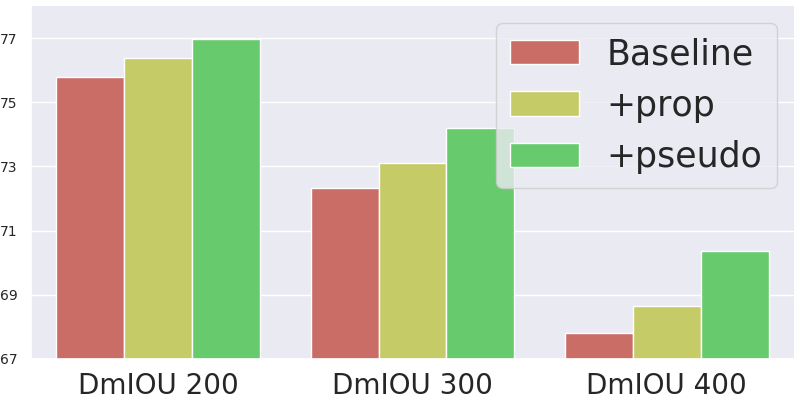
\includegraphics[height=0.4\linewidth]{figures/dmiou.png}
% }%
% {%
%     \vspace{-0.3em}%
%     \caption{\small Measuring the improvement on Distance based mIoU by training on pseudo-labels.}
%     \label{fig: figure-label}
% }%
% \killfloatstyle\ttabbox[\Xhsize]
% {%
%     \begin{tabular}[t]{llcc}
%         \toprule
%         \multicolumn{2}{l}{} & mIOU & $\text{\tiny DmIOU}_{200}$ \\
%         \midrule
%         \multicolumn{2}{l}{Baseline} &  &\\
%         \multicolumn{2}{l}{Baseline + SDC} & &\\
%         \multicolumn{2}{l}{Baseline + LID} & & \\
%         \multicolumn{2}{l}{Baseline + GT} & & \\
%         \bottomrule
%     \end{tabular}
% }%
% {%
%     \caption{\small Benefit of training with pseudo-labels on ApolloScape Dataset}\label{tab: table-label}
% }%
% \end{floatrow}

% % \caption{\small \emph{Left:} The sequence error for SVHN multi-digit recognition
% % on crops of $64\times 64$ pixels (64px), and inflated crops of $128 \times 128$
% % (128px) which include more background. \textsuperscript{*}The best reported
% % result from \cite{Ba14} uses model averagin}
% % % }}%
% \vspace{-1em}
% \end{figure}

\begin{table}[t]
    \centering
    \caption{ We show the benefit of training with our pseudo-labels. We also show the benefit of modelling label uncertainty. In the above table,  $D_{\hat{L}seq}$ contains propagated labels and $D_{\hat{L}ps}$ contains pseudo-semantic labels (refer Section~\ref{subsec-alea}).
    }\label{tab_main_ablation}
    \begin{tabular}{llcc}
\toprule
\multicolumn{2}{c}{Dataset}& Loss & mean IOU  \\
\midrule
\multicolumn{2}{l}{$D_L$} & C.E. & 77.62\\
\multicolumn{2}{l}{$D_L$ + \cite{nvidia_cvpr19} ($\pm 2,4,6,8$)}& RLL &77.82  \\
\multicolumn{2}{l}{$D_L$ + Ours ($\pm [2,4,6,8])$}&$\mathtt{UAT}$ & 78.45  \\
\midrule
\multicolumn{2}{l}{$D_L$ + GT($\pm [2,4,6,8])$}& \cite{gal_main} & 77.82  \\
\bottomrule
    \end{tabular}
\end{table}
 
% \begin{table}[t]
% \begin{center}\small
% % \setlength{\tabcolsep}{3pt}
% \begin{tabular}[t]{lccc}
% %%%%%% Title row starts here
% \\
% % Temporary header Graph would be better! TBD
% \toprule
% \multicolumn{1}{l}{} & $\text{{\tiny DmIOU}}_{200}$ & $\text{\tiny DmIOU}_{300}$ & $\text{\tiny DmIOU}_{200}$ \\
% \midrule
% \multicolumn{1}{l}{Baseline} & 75.79 & 72.32 & 67.80\\
% \multicolumn{1}{l}{+ prop} & 76.37 & 73.10 & 68.66 \\
% \midrule
% \multicolumn{1}{l}{+pseudo} & 76.37 & 73.10 & 68.66 \\
% \bottomrule
% \end{tabular}
% \qquad\qquad \qquad\qquad
% % \hspace{-2em}
% % \vtop{
% % \vspace{-1em}
% % \hbox{
% % 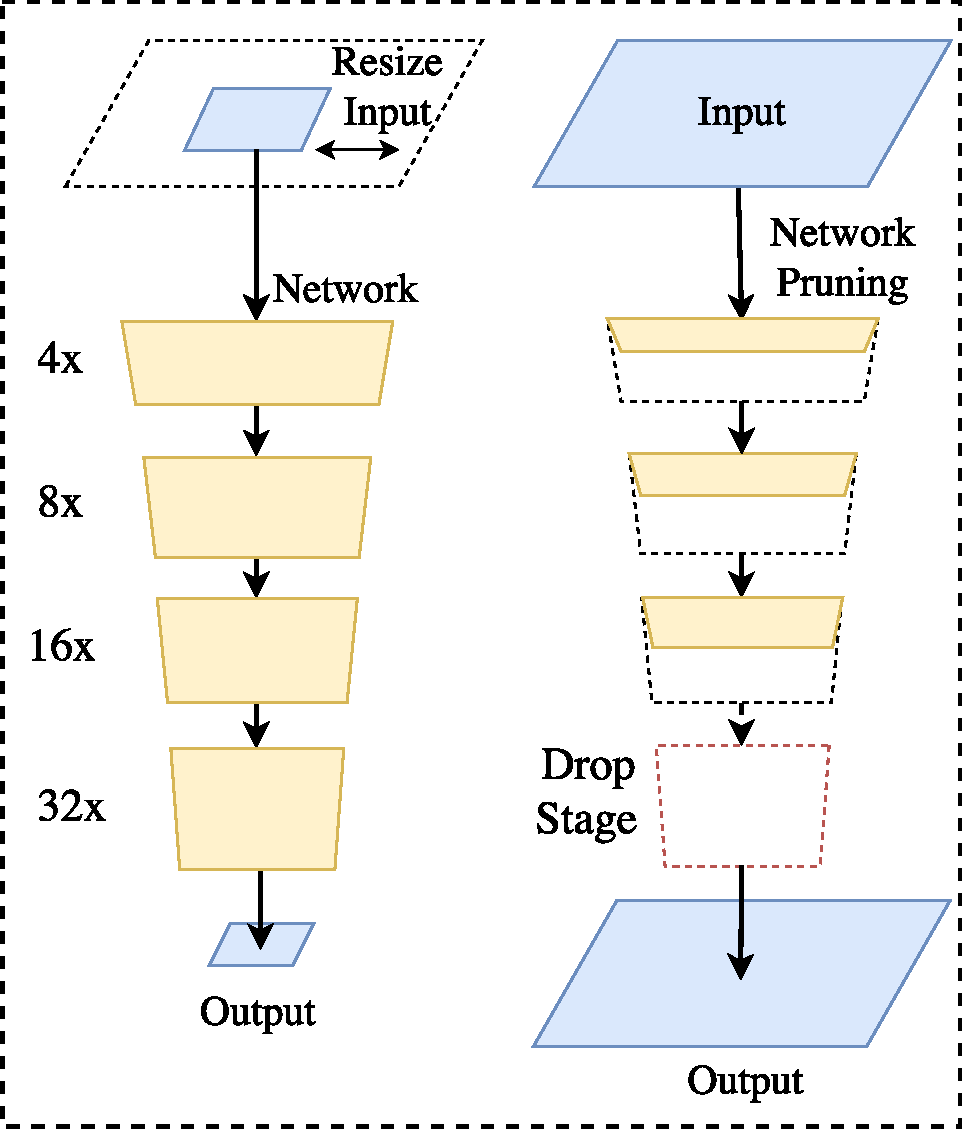
\includegraphics[width=0.6\textwidth]{figures/input_model.pdf}
% \begin{tabular}[t]{llcc}
% %%%%%% Title row starts here
% \toprule
% \multicolumn{2}{l}{} & mIOU & $\text{\tiny DmIOU}_{200}$ \\
% \midrule
% \multicolumn{2}{l}{Baseline} &  &\\
% \multicolumn{2}{l}{Baseline + SDC} & &\\
% \multicolumn{2}{l}{Baseline + LID} & & \\
% \multicolumn{2}{l}{Baseline + GT} & & \\
% \bottomrule
% \end{tabular}

% % }}%
% \end{center}
% \caption{\small \emph{Left:} The sequence error for SVHN multi-digit recognition
% on crops of $64\times 64$ pixels (64px), and inflated crops of $128 \times 128$
% (128px) which include more background. \textsuperscript{*}The best reported
% result from \cite{Ba14} uses model averagin}
% \label{table:svhn}
% \end{table}

% \let\clearpage\relax
% 
% \begin{table}[t]

% % \caption{\small \emph{Left:} The sequence error for SVHN multi-digit recognition
% % on crops of $64\times 64$ pixels (64px), and inflated crops of $128 \times 128$
% % (128px) which include more background. \textsuperscript{*}The best reported
% % result from \cite{Ba14} uses model averagin}
% % % }}%
% \vspace{-1em}
% \end{table}


\begin{table}[t]
\begin{center}\small
% \setlength{\tabcolsep}{3pt}
    \begin{tabular}{lc}
        \toprule
        \multicolumn{1}{c}{Method}& mean IOU  \\
        \midrule
        % DenseASPP \cite{Yang2018DenseASPP}&  80.6 \\
        % SPG  \cite{Cheng2019SPGNet}  &     $81.1$        \\
        % DANet  \cite{Fu2018DANet} &     $81.5$        \\
        HRNetv2  \cite{Sun2019HRNet}     &     $81.8$        \\
        EMANet  \cite{Li2019EMANet}&     $81.9$        \\
        ACNet \cite{Fu2019ACNet}&  \secbest{82.3}        \\
        \midrule
        Our Baseline  &     80.9        \\
        Ours WRP + UAT  &     \best{82.3}        \\
        \bottomrule
    \end{tabular}
\qquad\qquad \qquad\qquad
% \hspace{-2em}
% \vtop{
% \vspace{-1em}
% \hbox{
% 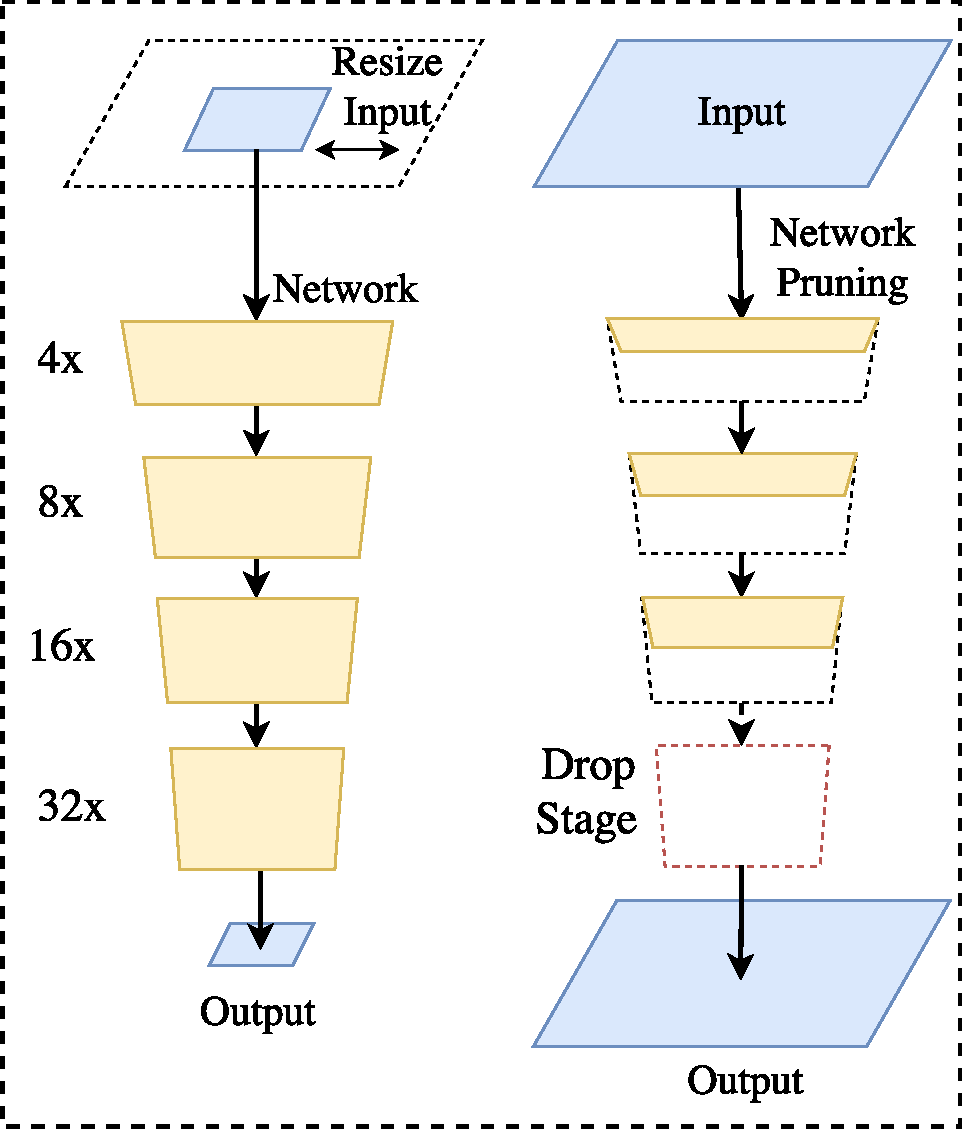
\includegraphics[width=0.6\textwidth]{figures/input_model.pdf}
    \begin{tabular}{llcc}
        \toprule
        \multicolumn{2}{c}{Dataset}& Loss & mean IOU  \\
        \midrule
        \multicolumn{2}{l}{$D_L$} & C.E. & 77.62\\
        \multicolumn{2}{l}{$D_L$ + \cite{nvidia_cvpr19} ($\pm 2,4,6,8$)}& RLL &77.82  \\
        \multicolumn{2}{l}{$D_L$ + Ours ($\pm [2,4,6,8])$}&$\mathtt{UAT}$ & 78.45  \\
        \midrule
        \multicolumn{2}{l}{$D_L$ + GT($\pm [2,4,6,8])$}& \cite{gal_main} & 77.82  \\
        \bottomrule
    \end{tabular}

% }}%
\end{center}
\caption{\small \emph{Left:} The sequence error for SVHN multi-digit recognition
on crops of $64\times 64$ pixels (64px), and inflated crops of $128 \times 128$
(128px) which include more background. \textsuperscript{*}The best reported
result from \cite{Ba14} uses model averagin}
\label{table:svhn}
\end{table}

% Can also have just one table


To benefit from propagated data, we find it essential to include propagated samples from multiple timesteps. Following~\cite{lp_eccv}, for each label in $D_L$, we include propagated labels at timesteps $t \pm p$ where $p \in \{2,4,6,8\}$ from $D_{\hat{L}seq}$. Furthermore, we include pseudo-labelling on the \texttt{train\_extra} subset $D_{\hat{L}ps}$ as well. The results are shown in Table~\ref{tab_main_ablation}. The propagated labels, when used with the \emph{Uncertainty-Aware Training} (UAT), enable us to boost the performance $0.49$ mIoU. The performance is further boosted by $0.47$ mIOU when $D_{\hat{L}ps}$ is used as well. Note how UAT plays a crucial role in increasing performance in the presence of propagated labels.
%   While simply adding the generated labels is found to be useful, the improvement is constraint by the noise in these labels. Once we introduce the uncertainty based learning (section~\ref{subsec-alea}), we are able to boost the result further. 

Finally, using the same method, we show that it is able to improve the \textit{state-of-the-art} on Cityscapes (when training with fine labels only). Table~\ref{} shows the improvement by training with our method. We observe that in the presence of coarse labels, and Mapillary Vistas pretraining~\cite{mapillary}, the benefits of label propagation are not clear (shown in supplementary). This is expected as label propagation cannot be performed for the coarse labels and the Mapillary Vistas dataset and hence, in the presence of those labels, propagation is performed for only $\sim$ 10\% of the entire dataset.

% \textbf{Stronger Metric}: Following~\cite{gated_iccv2019}, we also evaluate the distance-based mIoU, which measures performance on objects far away from the camera, which is much harder. The results are shown in Table~\ref{}, showing that the generated labels significantly help with objects further away.
% As the performance in Cityscapes dataset is found to be saturating, we find mIOU to be a insufficient metric to show improvements in performance. 
%Table~\ref{} compares our results with previous methods and show that the 0.6 \% improvement in mIOU translates to significant improvement in segmentation of objects far from the camera. 


\textbf{Evaluation on ApolloScape}: In Table~\ref{} we show the benefit of training with propagated labels and the uncertainty-aware training regime on Apolloscape dataset. %We find a improvment of x\% mIOU over the baseline using our labels and uncertainty based training.

\textbf{Modelling Label Noise with Uncertainty}: We demonstrate that the uncertainty estimates are able to model the noise in the data-generation process. Figure~\ref{} shows the precision-recall curves between the generated label $D_{\hat{L}seq}$ and manually annotated labels $D_{Lseq}$ on ApolloScape. % They show that the uncertainty is higher for noisy propagated labels. % label quality improves by removing labels with uncertainty larger than various percentile thresholds.



% What are the experiements: 
% 1) Apolloscapes  ppa/miou graph + examples on right. => By 25th
% 2) Previous dont work + uncertainty plot. 
% 2) Ablation ours Big table
% 3) Big table test on Cityscapes. Fine Only with All. =. End moment
% 4) L:Apolloscapes table mIOU. R: Finer metrics on Cityscapes.  = L: 27th, R: 23rd

% Supplementary: 
% 1) Failure all put in nvidia
% 2) All put in ours (val and test?)
% 3) propagation ablations.
% 4) Proof
% 5) Video
% 6) More image examples. 


% \section{Discussion}
% \label{section-discussion}
% 

Implications of the noise modelling. Essentially opening up the space of augmentation methods. 




\section{Conclusion}
\label{section-conclusion}

In this work, we address two questions: \emph{how to propagate labels}, and \emph{how to train with noisy pseudo-labels}. Our propagation method utilizes the concept of cycle consistency of labels to significantly improve label propagation. Further, our noisy label learning approach effectively utilizes uncertainty to alleviate the drawbacks of training with noisy labels. Using the proposed ingredients, we achieve state-of-the-art performance on Cityscapes. The noisy label learning approach opens the door to utilizing more noisy augmentation processes such as image-based rendering methods~\cite{}, and in the future, we hope to extend our work in that direction.


\newpage
\section*{Potential Broader Impact}
This research can be beneficial to companies or institutions requiring applications for semantic understanding of video data such as autonomous driving.
% We should mention that it can make semantic segmentation more accessible for people without resources to annotate large amount of data. 
% In Drawback I think we should mention that it does take more time to train --> more pollution and environmental cost. 
% 
If autonomous driving becomes an ubiquitous reality, humans currently working with manual car driving labor could be at disadvantage from the results of this research, although indirectly.
If an autonomous driving system fails due to the proposed component, the consequence could be an accident or the loss of human life.
We believe our proposed method leverages some bias in the data, as the data distribution of the training set will affect the type of representations that can be learned by the downstream semantic segmentation network.
% Instructions:
%Ethical aspects. Future societal consequences.
%Discuss both positive and negative outcomes.
%Must discuss the below:
% a) who may benefit from this research
% b) who may be put at disadvantage from this research
% c) what are the consequences of failure of the system
% d) whether the task/method leverages biases in the data.

% \section*{Acknowledgments and Disclosure of Funding}

% ---- Bibliography ----
%
% BibTeX users should specify bibliography style 'splncs04'.
% References will then be sorted and formatted in the correct style.
%
% \bibliographystyle{splncs04}
% \bibliographystyle{splncs03}
\bibliographystyle{ieee}
\bibliography{egbib}
% \bibliography{eccv2020kit/egbib}
\end{document}
